\documentclass{article}
\RequirePackage{etex}
\usepackage{geometry}
\geometry{a4paper, margin = 1.0in}
\usepackage[utf8]{inputenc}
\usepackage[english]{babel}
\usepackage[dvipsnames]{xcolor}
\usepackage{framed,graphicx}
\usepackage{hyperref}
\hypersetup{colorlinks=true,linkcolor=blue,filecolor=magenta,urlcolor=Cerulean,citecolor=SkyBlue}
\usepackage{listings}
\usepackage{mathtools}
\usepackage{amsfonts,amsthm,esint,mathrsfs}
\usepackage{paracol}
\usepackage{wrapfig}
\usepackage[nottoc]{tocbibind}
\usepackage{natbib}
\usepackage[font={scriptsize,it}]{caption}
\usepackage{float}
\usepackage{multicol}
\usepackage[font={scriptsize}]{subcaption}
\usepackage{pgfplots,tikz,tkz-euclide}
\usetikzlibrary{calc,patterns,angles,quotes,arrows,arrows.meta,shapes,shapes.geometric,cd,hobby,positioning}
\usetkzobj{all}
\pgfplotsset{compat=1.9}
\usepackage[toc,acronym,nogroupskip]{glossaries}
\usepackage{enumitem}
\usepackage{upgreek}
\graphicspath{{images/}}
%-------------Tikz Presets----------%
\pgfdeclareradialshading{myring}{\pgfpointorigin}{
color(0cm)=(transparent!0);
color(5mm)=(pgftransparent!50);
color(1cm)=(pgftransparent!100)}
\pgfdeclarefading{ringo}{\pgfuseshading{myring}}
%------------Theorem Styles---------%
\newtheoremstyle{mystyle}{\topsep}{\topsep}{}{}{\bfseries}{}{.5em}{}
\theoremstyle{mystyle}
\newtheorem{theorem}{Theorem}[section]
\newtheorem{definition}{Definition}[section]
\newtheorem{lemma}{Lemma}[section]
\newtheorem{corollary}{Corollary}[section]
\newtheorem{proposition}{Proposition}[section]
\newtheorem{example}{Example}[section]
\newtheorem{problem}{Problem}[section]
\newtheorem{question}{Question}[section]
\newtheorem{remark}{Remark}[section]
\newtheorem{properties}{Properties}[section]
\newtheorem{notation}{Notation}[section]
\newtheorem{axiom}{Axiom}[section]
\newtheorem*{theorem*}{Theorem}
\newtheorem*{definition*}{Definition}
\newtheorem*{properties*}{Properties}
\newtheorem*{remark*}{Remark}
%--------Declared Math Operators----%
\DeclareMathOperator{\Refl}{Refl}
\DeclareMathOperator{\Span}{Span}
\DeclareMathOperator{\sgn}{sgn}
\DeclareMathOperator{\multideg}{mutlideg}
\DeclareMathOperator{\LC}{LC}
\DeclareMathOperator{\LT}{LT}
\DeclareMathOperator{\LM}{LM}
\DeclareMathOperator{\LCM}{LCM}
\DeclareMathOperator{\Mon}{Mon}
\DeclareMathOperator{\Spec}{Spec}
\DeclareMathOperator{\proj}{proj}
\DeclareMathOperator{\comp}{comp}
\DeclareMathOperator{\sinc}{sinc}
%-------------New Commands----------%
\DeclarePairedDelimiter\norm{\lVert}{\rVert}
\DeclarePairedDelimiter\ceil{\lceil}{\rceil}
\DeclarePairedDelimiter\floor{\lfloor}{\rfloor}
\definecolor{shadecolor}{gray}{0.9}
\renewcommand*{\glstextformat}[1]{\textcolor{RoyalBlue}{#1}}
\renewcommand{\glsnamefont}[1]{\textbf{#1}}
\renewcommand\labelitemii{$\circ$}
\renewcommand\thesubfigure{\arabic{chapter}.\arabic{figure}.\arabic{subfigure}}
%---------------GLOSSARY------------%
\makeglossaries
\loadglsentries{glossary}
\loadglsentries{acronym}

\title{Surgery Theory}
\author{Ryan Maguire}
\date{\vspace{-5ex}}
\begin{document}
\maketitle
\tableofcontents
\setlength{\parindent}{0em}
\setlength{\parskip}{0em}
\section{Lecture Notes}
\subsection{Lecture 1: Homotopy}
\begin{wrapfigure}[8]{l}{0.35\textwidth}
    \centering
    \vspace{-2ex}
    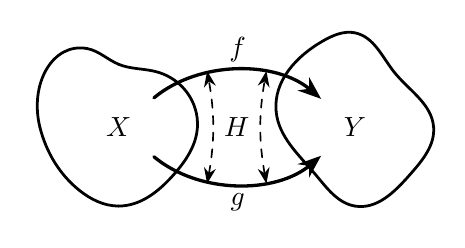
\begin{tikzpicture}[line width=1pt,line cap = round,>={Stealth[black]},every edge/.style={draw=black,very thick}]
        \node[fill=black,circle,inner sep=0pt,outer sep=0pt] at (0,0) (a) {};
        \node[fill=black,circle,inner sep=0pt,outer sep=0pt] at (-0.5,0.2) (b) {};
        \node[fill=black,circle,inner sep=0pt,outer sep=0pt] at (-1,1) (c) {};
        \node[fill=black,circle,inner sep=0pt,outer sep=0pt] at (-0.4,2) (d) {};
        \node[fill=black,circle,inner sep=0pt,outer sep=0pt] at (0, 1.8) (e) {};
        \node[fill=black,circle,inner sep=0pt,outer sep=0pt] at (0.5, 1.7) (f) {};
        \node[fill=black,circle,inner sep=0pt,outer sep=0pt] at (1,1) (g) {};
        \node[fill=black,circle,inner sep=0pt,outer sep=0pt] at (0.7,0.4) (h) {};
        \node at (0,1) (i) {$X$};
        \path[draw,use Hobby shortcut,closed=true](a) .. (b) .. (c) .. (d) .. (e) .. (f) .. (g) .. (h);
        \node[fill=black,circle,inner sep=0pt,outer sep=0pt] at (3,0) (a1) {};
        \node[fill=black,circle,inner sep=0pt,outer sep=0pt] at (2.5,0.4) (b1) {};
        \node[fill=black,circle,inner sep=0pt,outer sep=0pt] at (2,1.2) (c1) {};
        \node[fill=black,circle,inner sep=0pt,outer sep=0pt] at (2.6,2.1) (d1) {};
        \node[fill=black,circle,inner sep=0pt,outer sep=0pt] at (3, 2.2) (e1) {};
        \node[fill=black,circle,inner sep=0pt,outer sep=0pt] at (3.5, 1.7) (f1) {};
        \node[fill=black,circle,inner sep=0pt,outer sep=0pt] at (4,1) (g1) {};
        \node[fill=black,circle,inner sep=0pt,outer sep=0pt] at (3.7,0.4) (h1) {};
        \node at (3,1) (i1) {$Y$};
        \path[draw,use Hobby shortcut,closed=true](a1) .. (b1) .. (c1) .. (d1) .. (e1) .. (f1) .. (g1) .. (h1);
        \path[shorten >=0.2cm,shorten <=0.2cm,->] (i) edge[bend left=40] node[above] {$f$} (i1);
        \path[shorten >=0.2cm,shorten <=0.2cm,->] (i) edge[bend right=40] node[below] {$g$} (i1);
        \node at (1.5,1) (ho) {$H$};
        \node at (1.1,0.15) (t1) {};
        \node at (1.1,1.85) (t2) {};
        \node at (1.9,0.15) (t3) {};
        \node at (1.9,1.85) (t4) {};
        \path[draw=black,dashed,<->] (t1) edge[bend right =10,semithick] (t2);
        \path[draw=black,dashed,<->] (t3) edge[bend left =10,semithick] (t4);
    \end{tikzpicture}
    \caption[Surgery Theory - Homotopy Diagram]{Diagram for a homotopy between two functions $f,g:X\rightarrow Y$. $H$ `bends' $f$ into $g$, and vice-versa.}
    \label{fig:surgery_theory_course_homotopy_diagram_for_depicting_what_a_homotopy_is}
\end{wrapfigure}
Let $X$ and $Y$ be topological spaces, and let $f:X\rightarrow Y$ and $g:X\rightarrow Y$ be continuous functions. We now define what it means for $f$ and $g$ to be \textit{homotopic}.
\begin{definition}
A homotopy between continuous functions $f,g:X\rightarrow Y$ is a continuous function $H:X\times I \rightarrow Y$ such that $H(x,0)=f(x)$ and $H(x,1) = g(x)$.
\end{definition}
\begin{definition}
Homotopic functions, denoted $f\simeq g$, are continuous functions $f,g:X\rightarrow Y$ with a homotopy between them.
\end{definition}
\begin{notation}
The set of continuous functions $f:X\rightarrow Y$ is denoted $C(X,Y)$.
\end{notation}
\begin{example}
Let $X = \mathbb{R}^{n}$ and $Y = \mathbb{R}^{m}$, where $n,m\in \mathbb{N}$. Let $f,g:\mathbb{R}^{n}\rightarrow \mathbb{R}^{m}$ be arbitrary continuous functions. The `straight line' homotopy is a homotopy between any such functions. Let $H:\mathbb{R}^{n}\times I \rightarrow \mathbb{R}^{m}$ be defined by $H(x,t) = (1-t)f(x)+tg(x)$. Then $H(x,0) = f(x)$, and $H(x,1) = g(x)$. Moreover, $H$ is continuous. So $H$ is a homotopy between $f$ and $g$, and $f$ and $g$ are homotopic. Note that $g(x) = constant$ is possible. Any continuous function $f:\mathbb{R}^{n}\rightarrow\mathbb{R}^{m}$ is homotopic to a point.
\end{example}
\par
\begin{wrapfigure}[10]{r}{0.35\textwidth}
    \centering
    \vspace{-4ex}
    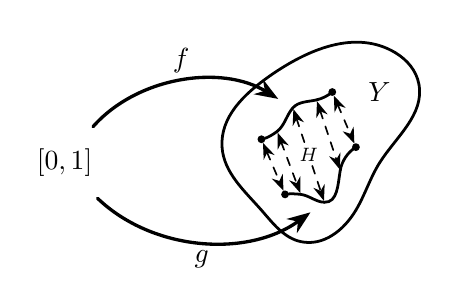
\begin{tikzpicture}[line width=1pt,line cap = round,>={Stealth[black]},every edge/.style={draw=black,very thick}]
        \node[fill=black,circle,inner sep=1pt,outer sep=0pt] at (2.5,1.3) (a0) {};
        \node[fill=black,circle,inner sep=0pt,outer sep=0pt] at (2.7,1.4) (b0) {};
        \node[fill=black,circle,inner sep=0pt,outer sep=0pt] at (2.9,1.7) (c0) {};
        \node[fill=black,circle,inner sep=0pt,outer sep=0pt] at (3.2,1.8) (d0) {};
        \node[fill=black,circle,inner sep=1pt,outer sep=0pt] at (3.4,1.9) (e0) {};
        \draw (a0) to [quick curve through={(b0) .. (c0) .. (d0)}] (e0);
        \node[fill=black,circle,inner sep=1pt,outer sep=0pt] at (2.8,0.6) (a1) {};
        \node[fill=black,circle,inner sep=0pt,outer sep=0pt] at (3,0.6) (b1) {};
        \node[fill=black,circle,inner sep=0pt,outer sep=0pt] at (3.3,0.5) (c1) {};
        \node[fill=black,circle,inner sep=0pt,outer sep=0pt] at (3.5,0.9) (d1) {};
        \node[fill=black,circle,inner sep=1pt,outer sep=0pt] at (3.7,1.2) (e1) {};
        \draw (a1) to [quick curve through={(b1) .. (c1) .. (d1)}] (e1);
        \path[draw=black,dashed,<->] (a0) edge[semithick] (a1);
        \path[draw=black,dashed,<->] (b0) edge[semithick] (b1);
        \path[draw=black,dashed,<->] (c0) edge[semithick] node[inner sep=0pt,outer sep=0pt,fill=white] {\scriptsize{\textit{H}}} (c1);
        \path[draw=black,dashed,<->] (d0) edge[semithick] (d1);
        \path[draw=black,dashed,<->] (e0) edge[semithick] (e1);
        \node[fill=black,circle,inner sep=0pt,outer sep=0pt] at (3,0) (a2) {};
        \node[fill=black,circle,inner sep=0pt,outer sep=0pt] at (2.5,0.4) (b2) {};
        \node[fill=black,circle,inner sep=0pt,outer sep=0pt] at (2,1.2) (c2) {};
        \node[fill=black,circle,inner sep=0pt,outer sep=0pt] at (2.6,2.1) (d2) {};
        \node[fill=black,circle,inner sep=0pt,outer sep=0pt] at (4.2, 2.4) (e2) {};
        \node[fill=black,circle,inner sep=0pt,outer sep=0pt] at (4.5, 2) (f2) {};
        \node[fill=black,circle,inner sep=0pt,outer sep=0pt] at (4,1) (g2) {};
        \node[fill=black,circle,inner sep=0pt,outer sep=0pt] at (3.7,0.4) (h2) {};
        \node at (0,1) (i) {$[0,1]$};
        \node at (4,1.9) (i1) {$Y$};
        \path[draw,use Hobby shortcut,closed=true](a2) .. (b2) .. (c2) .. (d2) .. (e2) .. (f2) .. (g2) .. (h2);
        \path[shorten >=0.2cm,shorten <=0.2cm,->] (i) edge[bend left=40] node[above] {$f$} (c0);
        \path[shorten >=0.2cm,shorten <=0.2cm,->] (i) edge[bend right=40] node[below] {$g$} (c1);
    \end{tikzpicture}
    \caption[Surgery Theory - Homotopy Diagram]{Diagram for the straight-line homotopy between functions $f,g:[0,1]\rightarrow Y$.}
    \label{fig:surgery_theory_course_homotopy_diagram_for_straight_line_homotopy}
\end{wrapfigure}
Figure \ref{fig:surgery_theory_course_homotopy_diagram_for_depicting_what_a_homotopy_is} shows two topological spaces and two continuous functions $f,g:X\rightarrow Y$. The homotopy $H$ `bends' $f$ into $g$, and vice-versa. One can visualize a homotopy by letting $X = [0,1]$, and $Y\subset \mathbb{R}^{2}$ be a nice blob, like the one shown in Fig.~\ref{fig:surgery_theory_course_homotopy_diagram_for_straight_line_homotopy}. Let $f:[0,1]\rightarrow Y$ and $g:[0,1]\rightarrow Y$ be smooth curves within the blob. $H(x,t) = (1-t)f(x)+tg(x)$ is the map that drags $f(x)$ to $g(x)$ via the straight line connecting the two points. This is done for every point $x\in [0,1]$. The next thing to show is that the notion of homotopy $\simeq$ is an equivalence relation on the set of continuous functions from $X$ to $Y$, $C(X,Y)$.
\begin{theorem}
Homotopic is an equivalence relation on $C(X,Y)$.
\end{theorem}
\begin{proof}
We must show that $\simeq$ is reflexive, symmetric, and transitive.
\begin{enumerate}
    \item $\simeq$ is reflexive. If $f\in C(X,Y)$, then let $H(x,t) = f(x)$. Then $H:X\times I \rightarrow Y$ is a continuous function, $H(x,0) = f(x)$, and $H(x,1) = f(x)$. Thus, $H$ is a homotopy between $f$ and itself. $f\simeq f$.
    \item $\simeq$ is symmetric. If $f,g\in C(X,Y)$ and $f\simeq g$, then there exists an $H:X\times I \rightarrow Y$ such that $H(x,0) = f(x)$ and $H(x,1) = g(x)$. Let $G(x,t) = F(x,1-t)$. But $(x,t)\mapsto (x,1-t)$ is a continuous mapping, and the composition of continuous functions is continuous, and therefore $G(x,t)$ is continuous. Moreover, $G(x,0) = H(x,1) = g(x)$, and $F(x,1) = G(x,0) = f(x)$. Therefore, $g\simeq f$.
    \item $\simeq$ is transitive. If $f,g,h\in C(X,Y)$, $f\simeq g$, and $g\simeq h$, then there exists $H_{1}(x,t)$ such that $H_{1}(x,0) = f(x)$ and $H_{1}(x,1) = g(x)$, and there exists $H_{2}(x,t)$ such that $H_{2}(x,0) = g(x)$ and $H_{2}(x,1) = h(x)$. Let $H:X\times I\rightarrow Y$ be defined by
    \begin{equation*}
        H_{3}(x,t) = \begin{cases} H_{1}(x,2t), & 0\leq t\leq \frac{1}{2}\\ H_{2}(x,2t-1), & \frac{1}{2}<t\leq 1 \end{cases}
    \end{equation*}
    Then, by the pasting lemma, $H_{3}(x,t)$ is continuous. But $H_{3}(x,0) = H_{1}(x,0) = f(x)$, and $H_{3}(x,1) = H_{2}(x,1) = h(x)$. Therefore, $f\simeq h$.
\end{enumerate}
\end{proof}
\begin{definition}
Homotopy equivalent spaces are topological spaces $X,Y$ such that there exists functions $f\in C(X,Y)$ and $g\in C(Y,X)$ such that $f\circ g \simeq id_{Y}$, and $g\circ f \simeq id_{X}$.
\end{definition}
\begin{definition}
A homotopy equivalence from a topological space $X$ to a topological space $Y$ is a function $f\in C(X,Y)$ such that there exists a function $g\in C(Y,X)$ such that $f\circ g \simeq id_{Y}$, $g\circ f \simeq id_{X}$.
\end{definition}
\begin{definition}
A homotopy inverse of a homotopy equivalence $f\in C(X,Y)$ is a function $g\in C(Y,X)$ such that $f\circ g \simeq id_{Y}$ and $g\circ f \simeq id_{X}$.
\end{definition}

\begin{definition}
A homeomorphism from a topological space $X$ to a topological space $Y$ is a continuous bijection $f:X\rightarrow Y$ such that $f^{-1}:Y\rightarrow X$ is continuous.
\end{definition}
\begin{definition}
Homeomorphic topological spaces are topological spaces $X$ and $Y$ such that there exists a homeomorphism $f:X\rightarrow Y$ between them.
\end{definition}
\begin{theorem}
\label{theorem:surgery_theory_homeomorphic_implies_homotopy_equivalent}
If $X$ and $Y$ are homeomorphic, then they are homotopy equivalent.
\end{theorem}
\begin{proof}
If $X$ and $Y$ are homeomorphic, then there is a homeomorphism $f:X\rightarrow Y$. But then $f$ is a continuous map from $X$ to $Y$, and $f^{-1}$ is a continuous map from $Y$ to $X$. Moreover, $f\circ f^{-1} = id_{Y}$, and $f^{-1}\circ f = id_{X}$, for $f$ is a bijection. But $id_{X}\simeq id_{X}$, and $id_{Y}\simeq id_{Y}$. Therefore $X$ and $Y$ are homotopy equivalent.
\end{proof}
The study of surgery theory ask about the converse of theorem \ref{theorem:surgery_theory_homeomorphic_implies_homotopy_equivalent}. The converse of this theorem is not always true, as we will now demonstrate.
\begin{theorem}
\label{theorem:surgery_theory_homotopic_does_not_imply_homeomorphic}
There exist homotopy equivalent spaces that are not homeomorphic.
\end{theorem}
\begin{proof}
For let $X=\mathbb{R}^{2}$, and $Y = \{(0,0)\}$. Let $f:X\rightarrow Y$ be defined by $f(x,y) = (0,0)$. Let $g:Y\rightarrow X$ be defined by $g(x,y) = (x,y)$. Let $H_1(x,y,t) = (1-t)(x,y)$. Then $H_{1}$ is continuous, $H_{1}(x,y,0) = (x,y)$, and $H_{1}(x,y,0) = (0,0)$. Thus, $H_{1}$ is a homotopy between $g\circ f$ and $id_{X}$, and therefore $g\circ f \simeq id_{X}$. But also $f\circ g = id_{Y}$, and $id_{Y}\simeq id_{Y}$. Therefore $X$ and $Y$ are homotopy equivalent. But there is no homeomorphism from $X$ to $Y$. For suppose not. If $h:X\rightarrow Y$ is a homeomorphism, then it is a bijection. But if $h$ is a bijection, then $|X| = |Y|$. But $\mathbb{R}^2$ is uncountable, and $|Y| = 1$. A contradiction. Thus, $X$ and $Y$ are not homeomorphic.
\end{proof}
\begin{wrapfigure}[6]{r}{0.35\textwidth}
    \centering
    \vspace{-5ex}
    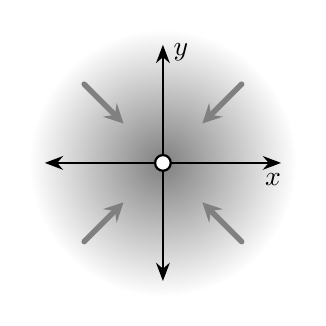
\begin{tikzpicture}[line width=1pt,line cap = round,>={Stealth[black]},every edge/.style={draw=black,very thick}]
        \filldraw[even odd rule,inner color=gray,outer color=white,draw=white] (0,0) circle (1.7);
        \draw[thick, <->] (-1.5,0) -- (1.5,0);
        \draw[thick, <->] (0,-1.5) -- (0,1.5);
        \draw[>=stealth,fill=gray,draw=gray,line width = 0.7mm,->](1,1) --++ (-0.5,-0.5);
        \draw[>=stealth,fill=gray,draw=gray,line width = 0.7mm,->](-1,-1) --++ (0.5,0.5);
        \draw[>=stealth,fill=gray,draw=gray,line width = 0.7mm,->](1,-1) --++ (-0.5,0.5);
        \draw[>=stealth,fill=gray,draw=gray,line width = 0.7mm,->](-1,1) --++ (0.5,-0.5);
        \node[fill=white,circle,thick, draw,inner sep=2pt,outer sep=3pt] at (0,0) (O) {};
        \node at (1.4,0) [below] {$x$};
        \node at (0,1.4) [right] {$y$};
    \end{tikzpicture}
    \vspace{-1ex}
    \caption{Retraction of $\mathbb{R}^{2}$ to $(0,0)$}
    \label{fig:surgery_theory_course_homotopy_equivalence_diagram_of_plane_with_point}
\end{wrapfigure}
Fig.~\ref{fig:surgery_theory_course_homotopy_equivalence_diagram_of_plane_with_point} shows the mapping $f$ between $\mathbb{R}^{2}$ and $\{(0,0)\}$. Theorem \ref{theorem:surgery_theory_homotopic_does_not_imply_homeomorphic} relies on the fact that $\mathbb{R}^2$ and $\{(0,0)\}$ are of different \textit{cardinality}. However, even if the topological spaces $X$ and $Y$ are homotopy equivalent, and are of the same cardinality, it is still possible that they are not homeomorphic.
\begin{theorem}
\label{theorem:surgery_theory_Homotopy_equivalance_of_plane_without_point_and_unit_disc_but_not_homeomorphic}
$\mathbb{R}^{2}\setminus\{(0,0)\}$ is homotopy equivalent to $S^{1}$, but not homeomorphic.
\end{theorem}
\begin{proof}
For let $X = \mathbb{R}^{2}\setminus\{(0,0)\}$, and let $Y = S^{1} = \{(x,y)\in \mathbb{R}^{2}:x^2+y^2=1\}$. Let $f:X\rightarrow Y$ be defined by $f(x,y) = \frac{(x,y)}{\norm{(x,y)}}$. Let $g:Y\rightarrow X$ be defined by $g(x,y) = (x,y)$. Let $H_1(x,y,t) = (1-t)\frac{(x,y)}{\norm{(x,y)}}+t(x,y)$. But then $H_1(x,y,0) = \frac{(x,y)}{\norm{x,y}}$, and $H_1(x,y,1) = (x,y)$. Thus $H_1$ is a homotopy between $g\circ f$ and $id_{X}$. But also $(f\circ g)(x,y) = (x,y)$, for all $(x,y)\in S^{1}$. Therefore $f\circ g= id_{Y}$, and $id_{Y}\simeq id_{Y}$. Therefore, $X$ and $Y$ are homotopy equivalent. However, $\dim(X) = 2$ and $\dim(Y) = 1$. But homeomorphisms preserve dimension. Therefore, $X$ and $Y$ are not homeomorphic.
\end{proof}
\begin{figure}[H]
    \centering
    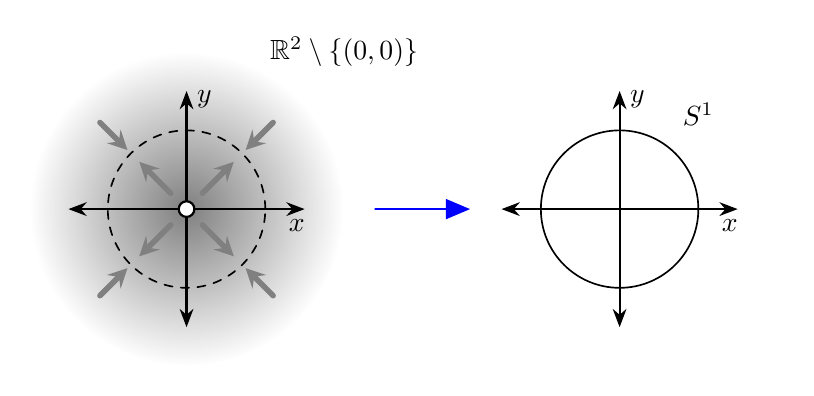
\begin{tikzpicture}[line width=1pt,line cap = round,>={Stealth[black]},every edge/.style={draw=black,very thick}]
        \filldraw[even odd rule,inner color=gray,outer color=white,draw=white] (0,0) circle (2);
        \draw[thick, <->] (-1.5,0) -- (1.5,0);
        \draw[thick, <->] (0,-1.5) -- (0,1.5);
        \draw[>=stealth,fill=gray,draw=gray,line width = 0.7mm,->](1.1,1.1) --++ (-0.35,-0.35);
        \draw[>=stealth,fill=gray,draw=gray,line width = 0.7mm,->](-1.1,-1.1) --++ (0.35,0.35);
        \draw[>=stealth,fill=gray,draw=gray,line width = 0.7mm,->](1.1,-1.1) --++ (-0.35,0.35);
        \draw[>=stealth,fill=gray,draw=gray,line width = 0.7mm,->](-1.1,1.1) --++ (0.35,-0.35);
        \draw[>=stealth,fill=gray,draw=gray,line width = 0.7mm,->](0.2,0.2) --++ (0.4,0.4);
        \draw[>=stealth,fill=gray,draw=gray,line width = 0.7mm,->](-0.2,-0.2) --++ (-0.4,-0.4);
        \draw[>=stealth,fill=gray,draw=gray,line width = 0.7mm,->](0.2,-0.2) --++ (0.4,-0.4);
        \draw[>=stealth,fill=gray,draw=gray,line width = 0.7mm,->](-0.2,0.2) --++ (-0.4,0.4);
        \draw[dashed,draw=black,semithick] (0,0) circle (1);
        \node[fill=white,circle,thick, draw,inner sep=2pt,outer sep=3pt] at (0,0) (O) {};
        \node at (1.4,0) [below] {$x$};
        \node at (0,1.4) [right] {$y$};
        \node at (2,2) {$\mathbb{R}^{2}\setminus \{(0,0)\}$};
        \draw[>=triangle 45,draw=blue,->](2.4,0) --++ (1.2,0);
        \draw[thick, <->] (4,0) -- (7,0);
        \draw[thick, <->] (5.5,-1.5) -- (5.5,1.5);
        \draw[draw=black,semithick] (5.5,0) circle (1);
        \node at (6.9,0) [below] {$x$};
        \node at (5.5,1.4) [right] {$y$};
        \node at (6.5,1.2) {$S^{1}$};
        \node at (7.5,0) {};
    \end{tikzpicture}
    \caption[Surgery Theory - HE From $\mathbb{R}^2\setminus\{(0,0)\}$ to $S^{1}$]{Homotopy Equivalence of $\mathbb{R}^{2}\setminus\{(0,0)\}$ and $S^{1}$}
    \label{fig:surgery_theory_homotopy_equivalence_between_the_plane_with_a_point_removed_and_the_unit_circle}
\end{figure}
Theorem \ref{theorem:surgery_theory_Homotopy_equivalance_of_plane_without_point_and_unit_disc_but_not_homeomorphic} relies on the fact that $\mathbb{R}^{2}\setminus \{(0,0)\}$ and $S^{1}$ are of different \textit{dimension}. However, even if $X$ and $Y$ are of the same cardinality \textit{and} of the same dimension, it is still possible that they are homotopy equivalent, but not homeomorphic. First, we show that $S^{2}\setminus \{(0,0,1)\}$ is homeomorphic to $D^{2}$.
\begin{theorem}
\label{theorem:surgery_theory_the_sphere_with_a_point_removed_is_homeomorphic_to_the_plane}
$S^{3}\setminus \{(0,0,1)\}$ is homeomorphic to $\mathbb{R}^{2}$
\end{theorem}
\begin{proof}
For let $f:S^{3}\setminus \{(0,0,1)\}\rightarrow \mathbb{R}^{2}$ be the stereographic projection mapping. That is, $f(x,y,z) = (\frac{x}{1-z},\frac{y}{1-z})$, for $(x,y,z)\in S^{2}\setminus \{(0,0,1)\}$. If $(X,Y) \in \mathbb{R}^{2}$, let:
\begin{equation*}
     x = \frac{2X}{\norm{(X,Y)}^{2}+1} \quad\quad y = \frac{2Y}{\norm{(X,Y)}^{2}+1}   \quad\quad z = \frac{\norm{(X,Y)}^{2}-1}{\norm{(X,Y)}^{2}+1} 
\end{equation*}
Then:
\begin{equation*}
    \bigg(\frac{x}{1-z},\frac{y}{1-z}\bigg) = \bigg(\frac{\frac{2X}{\norm{(X,Y)}^{2} + 1}}{\frac{2}{\norm{(X,Y)}^{2}+1}},\frac{\frac{2Y}{\norm{(X,Y)}^{2}+1}}{\frac{2}{\norm{(X,Y)}^{2}+1}}\bigg) = (X,Y)    
\end{equation*}
and
\begin{align*}
    \norm{(x,y,z)} &= \sqrt{\frac{4X^{2}}{\big(\norm{(X,Y)}^{2}+1\big)^{2}} + \frac{4Y^{2}}{\big(\norm{(X,Y)}^{2}+1\big)^{2}} + \frac{(\norm{(X,Y)}^{2}-1)^{2}}{(\norm{(X,Y)}^{2}+1)^{2}}}\\
    &= \sqrt{\frac{4\norm{(X,Y)}^{2} + \norm{(X,Y)}^{4} - 2\norm{(X,Y)}^{2} + 1}{(\norm{(X,Y)}+1)^{2}}}= \sqrt{\frac{\norm{(X,Y)}^{4} + 2\norm{(X,Y)}^{2} + 1}{(\norm{(X,Y)}^{2}+1)^{2}}}\\
    &= \sqrt{\frac{(\norm{(X,Y)}^{2}+1)^{2}}{(\norm{(X,Y)}^{2}+1)^{2}}}= 1
\end{align*}
Thus, $(x,y,z) \in S^{2}\setminus \{(0,0,1)\}$, and $f$ is surjective. If $f(x_1,y_1,z_1) = f(x_2,y_2,z_2)$, then $z_{1} = z_{2}$. For as $(x_1,y_1,z_1)\in S^{2}\setminus\{(0,0,1)\}$, and therefore $x_{1}^{2} + y_{1}^{2} = 1-z_{1}^{2}$, we have:
\begin{equation*}
    \norm{(X,Y)}^{2} = \frac{x_{1}^2+y_{1}^2}{(1-z_{1})^{2}} = \frac{1-z_{1}^{2}}{(1-z_{1})^{2}}
\end{equation*}
But:
\begin{equation*}
    \norm{(X,Y)}^{2} = \frac{x_{2}^{2}+y_{2}^{2}}{(1-z_{2})^{2}} = \frac{1-z_{2}^{2}}{(1-z_{2})^{2}}   
\end{equation*}
So we have $\frac{1-z_{1}^{2}}{(1-z_{1})^{2}} = \frac{1-z_{2}^{2}}{(1-z_{2})^{2}}$. Simplifying, we get $\frac{1+z_{1}}{1-z_{1}} = \frac{1+z_{2}}{1-z_{2}}$. But $f(x) = \frac{1+x}{1-x}$ is an injective function, and therefore $z_{1} = z_{2}$. From this:
\begin{equation*}
    \frac{x_{1}}{1-z_{1}} = \frac{x_{2}}{1-z_{2}} \Rightarrow x_{1} = x_{2}
\end{equation*}
Similarly, $y_{1} = y_{2}$. Thus, $f$ is injective. So $f$ is a bijection. Moreoever, $f$ is continuous as $\frac{x}{1-z}$ and $\frac{y}{1-z}$ are continuous. Finally:
\begin{equation*}
    f^{-1}(X,Y) = \bigg(\frac{2X}{\norm{(X,Y)}^{2}+1},\frac{2Y}{\norm{(X,Y)}^{2}+1},\frac{\norm{(X,Y)}^{2}-1}{\norm{(X,Y)}^{2}+1}\bigg)
\end{equation*}
Which is continuous. $f$ is a homeomorphism.
\end{proof}
Fig.~\ref{fig:surgery_theory_stereographic_projection_of_sphere_to_plane_homeomorphism} depicts the stereographic projection used to prove theorem \ref{theorem:surgery_theory_the_sphere_with_a_point_removed_is_homeomorphic_to_the_plane}. It can be seen that $(0,0,1)$ projects `to infinite'. Because of this, it is not uncommon to call this point infinity. Next, we prove that $\mathbb{R}^{2}$ is homeomorphic to $D^{2}$, almost completing our claim that $S^{2}\setminus \{(0,0,1)\}$ is homeomorphic to $D^{2}$.
\begin{theorem}
$\mathbb{R}^{2}$ is homeomorphic to $D^{2}$.
\end{theorem}
\begin{proof}
Let $f:D^{2}\rightarrow \mathbb{R}^{2}$ be defined by $f(\mathbf{x}) = \frac{\mathbf{x}}{1-\norm{\mathbf{x}}}$. $f$ is surjective. For $\mathbf{0}\mapsto \mathbf{0}$. If $\mathbf{y}\in \mathbb{R}^2\setminus \{\mathbf{0}\}$, then let $\mathbf{x} = \frac{\mathbf{y}}{1+\norm{\mathbf{y}}}$. Then $\norm{\mathbf{x}} = \frac{\norm{\mathbf{y}}}{1+\norm{\mathbf{y}}} < 1$, and thus $\mathbf{x}\in D^{2}$. But $f(\mathbf{x}) = \frac{\frac{\mathbf{y}}{1+\norm{\mathbf{y}}}}{1 - \frac{\norm{\mathbf{y}}}{1+\norm{\mathbf{y}}}} = \mathbf{y}$. $f$ is surjective. Moreover, $f$ is injective. For if $f(\mathbf{x}_{1}) = f(\mathbf{x}_{2})$, then $\frac{\norm{\mathbf{x}_{1}}}{1+\norm{\mathbf{x}_{1}}} = \norm{f(\mathbf{x}_{1})} = \norm{f(\mathbf{x}_{2})} = \frac{\norm{\mathbf{x}_{2}}}{1+\norm{\mathbf{x}}_{2}}$, and therefore $\norm{\mathbf{x}}_{1} = \norm{\mathbf{x}_{2}}$. But $\frac{\mathbf{x}_{1}}{1+\norm{\mathbf{x}_{1}}} = \frac{\mathbf{x}_{2}}{1+\norm{\mathbf{x}_{2}}}$, and therefore $\mathbf{x}_{1} = \mathbf{x}_{2}$. $f$ is bijective. Moreover, $f$ is continuous. Finally, $f^{-1}(\mathbf{y}) = \frac{\mathbf{y}}{1+\norm{\mathbf{y}}}$ is continuous. $f$ is a homeomorphism.
\end{proof}
\begin{figure}[t]
    \centering
    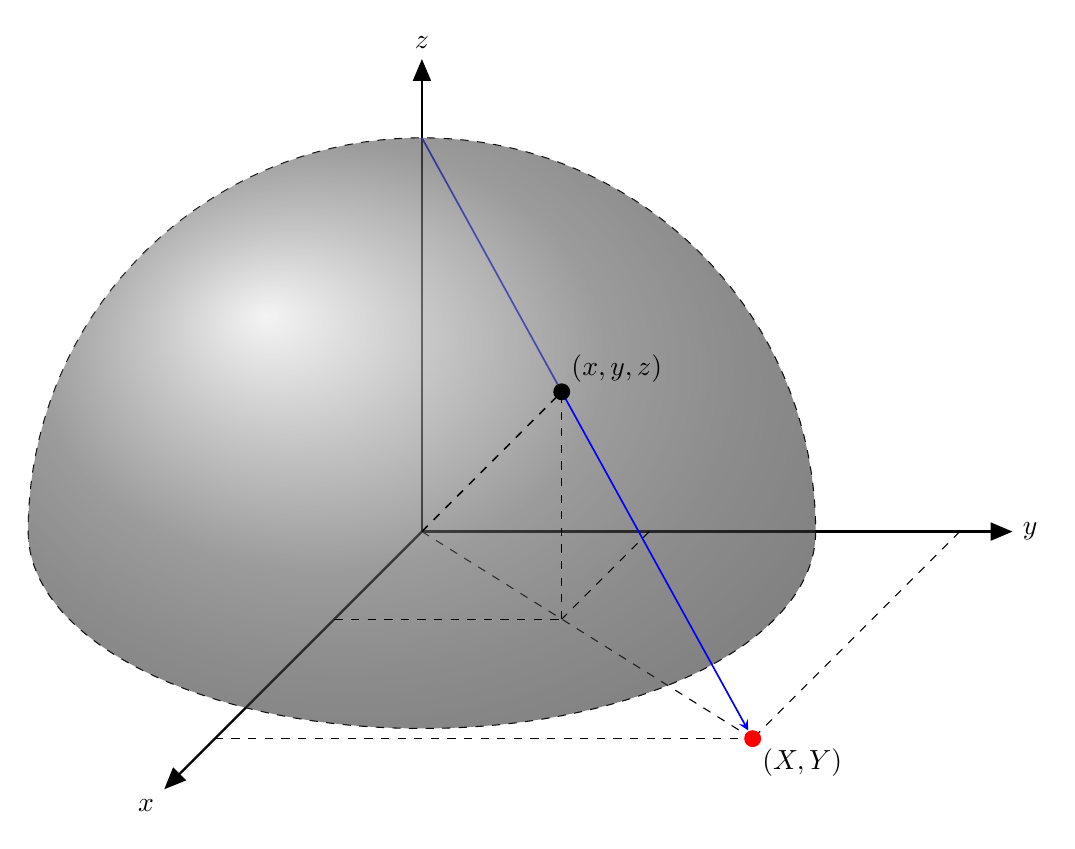
\begin{tikzpicture}[scale=5,>=triangle 45]
        %draw the main coordinate system axes
        \draw[thick,->] (0,0,0) -- (1.5,0,0) node[right]{$y$};
        \draw[thick,->] (0,0,0) -- (0,1.2,0) node[above]{$z$};
        \draw[thick,->] (0,0,0) -- (0,0,1.7) node[below left]{$x$};
        %draw some dashed arcs, demonstrating direct arc drawing
        \draw[dashed] (1cm,0) arc (0:-180:1cm and 5mm) arc (180:0:1cm and 1cm);
        \coordinate (A) at (0.57735026918962,0.57735026918962,0.57735026918962);
        \node[circle,inner sep=0pt, outer sep=1mm] (B) at (1.3660254037844,0,1.3660254037844) {};
        \draw[draw=blue,semithick] (0,1,0) -- (A);
        \draw[dashed] (0,0,0) -- (1.3660254037844,0,1.3660254037844);
        \shade[ball color=gray,opacity=0.6] (1cm,0) arc (0:-180:1cm and 5mm) arc (180:0:1cm and 1cm);
        \draw[draw=blue,semithick,>=stealth,->] (A) -- (B);
        \draw[dashed,thin] (0,0,1.3660254037844) -- (1.3660254037844,0,1.3660254037844);
        \draw[dashed,thin] (1.3660254037844,0,0) -- (1.3660254037844,0,1.3660254037844);
        \draw[dashed,semithick] (0,0,0) -- (0.57735026918962,0.57735026918962,0.57735026918962);
        \draw[dashed,thin]      (0,0,0.57735026918962) -- (0.57735026918962,0,0.57735026918962);
        \draw[dashed,thin]      (0.57735026918962,0,0) -- (0.57735026918962,0,0.57735026918962);
        \draw[dashed,thin]      (0.57735026918962,0,0.57735026918962) -- (0.57735026918962,0.57735026918962,0.57735026918962);
        \draw[dashed,thin]      (0,0,0.57735026918962) -- (0.57735026918962,0,0.57735026918962);
        \filldraw[black] (0.57735026918962,0.57735026918962,0.57735026918962) circle (0.2mm);
        \filldraw[red]   (1.3660254037844,0,1.3660254037844) circle (0.2mm);
        \node at (A) [above right] {$(x,y,z)$};
        \node at (B) [below right] {$(X,Y)$};
    \end{tikzpicture}
    \caption[Surgery Theory - Stereographic Projection]{Stereographic Projection of the Sphere onto the Plane}
    \label{fig:surgery_theory_stereographic_projection_of_sphere_to_plane_homeomorphism}
\end{figure}
\begin{theorem}
$S^{2}\setminus\{(0,0,1)\}$ is homeomorphic to $D^{2}$.
\end{theorem}
\begin{proof}
For $S^{2}\setminus\{(0,0,1)\}$ is homeomorphic to $\mathbb{R}^{2}$, and $\mathbb{R}^{2}$ is homeomorphic to $D^{2}$. But homeomorphism is an equivalence relation, so $S^{2}\setminus\{(0,0,1)\}$ is homeomorphic to $D^{2}$.
\end{proof}
\begin{figure}[H]
    \centering
    \resizebox{\textwidth}{!}{
    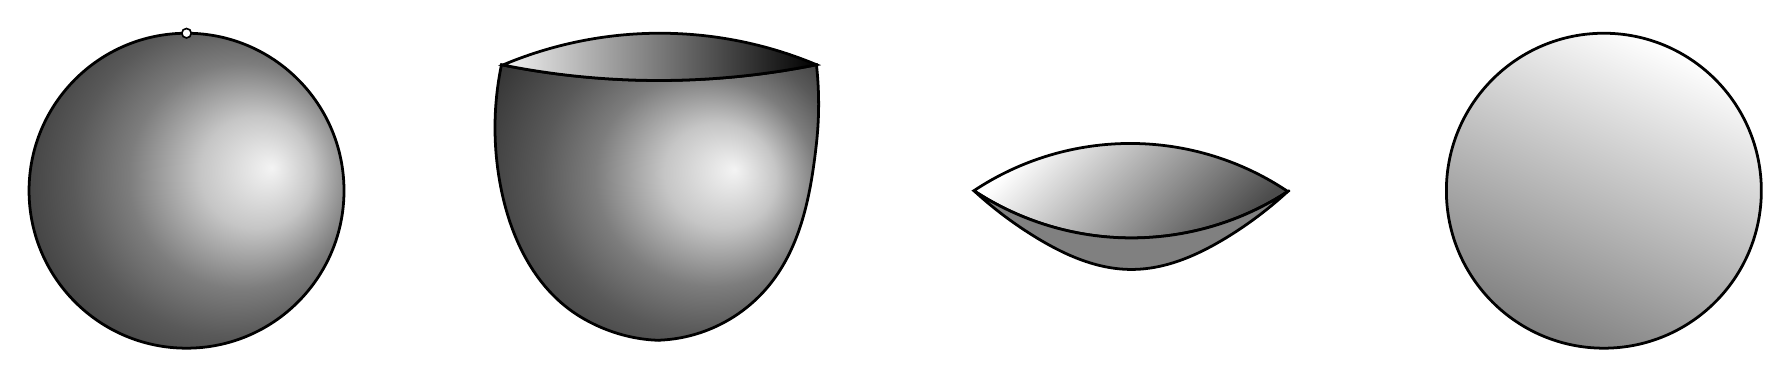
\begin{tikzpicture}[scale=2,line width=1pt,line cap = round,>={Stealth[black]},every edge/.style={draw=black,very thick}]
        \filldraw[ball color = gray!60!white,draw=black, shading angle = 240] (-4,0) circle (1);
        \filldraw[white,draw=black,semithick]   (-4,1) circle (0.3mm);
        \node[fill=black,circle,inner sep=0pt,outer sep=0pt] at (-1,-0.95) (a) {};
        \node[fill=black,circle,inner sep=0pt,outer sep=0pt] at (-1.5,-0.8) (b) {};
        \node[fill=black,circle,inner sep=0pt,outer sep=0pt] at (-2,0) (c) {};
        \node[fill=black,circle,inner sep=0pt,outer sep=0pt] at (-2,0.8) (d) {};
        \node[fill=black,circle,inner sep=0pt,outer sep=0pt] at (-1, 0.7) (e) {};
        \node[fill=black,circle,inner sep=0pt,outer sep=0pt] at (0, 0.8) (f) {};
        \node[fill=black,circle,inner sep=0pt,outer sep=0pt] at (-0,0.3) (g) {};
        \node[fill=black,circle,inner sep=0pt,outer sep=0pt] at (-0.3,-0.6) (h) {};
        \node[fill=black,circle,inner sep=0pt,outer sep=0pt] at (-1, 1) (top) {};
        \path[draw=black,ball color=gray!60!white, shading angle = 250 ] (a) to [quick curve through={(b) .. (c)}] (d) to [quick curve through={(e)}] (f) to [quick curve through={(g) .. (h)}] cycle;
        \path[draw=black,left color = white!90!gray, right color = black] (d) to [quick curve through={(e)}] (f) to [quick curve through={(top)}] cycle;
        \node[fill=black,circle,inner sep=0pt,outer sep=0pt] at (2,-0.5)     (a1) {};
        \node[fill=black,circle,inner sep=0pt,outer sep=0pt] at (1.4,-0.3) (b1) {};
        \node[fill=black,circle,inner sep=0pt,outer sep=0pt] at (1,0) (c1) {};
        \node[fill=black,circle,inner sep=0pt,outer sep=0pt] at (2,-0.3) (BOT1) {};
        \node[fill=black,circle,inner sep=0pt,outer sep=0pt] at (2,0.3) (TOP1) {};
        \node[fill=black,circle,inner sep=0pt,outer sep=0pt] at (3,0) (d1) {};
        \node[fill=black,circle,inner sep=0pt,outer sep=0pt] at (2.6,-0.3) (e1) {};
        \path[draw=black,left color=white, right color = white!30!black, shading angle = 45] (d1) to [quick curve through={(BOT1)}] (c1) to [quick curve through={(TOP1)}] cycle;
        \path[draw=black,fill=gray] (d1) to [quick curve through={(BOT1)}] (c1) to [curve through={(b1) (a1) (e1)}] cycle;
        \filldraw[draw=black,right color = white, left color = white!50!black,shading angle = 155] (5,0) circle (1);
    \end{tikzpicture}}
    \caption[Surgery Theory - Homeomorphism From $S^{2}\setminus\{(0,0,1)\}$ and $D^{2}$]{The unit sphere with a point removed can be continuously deformed into the open unit disc.}
    \label{fig:my_label}
\end{figure}
We can use the fact that $S^{2}\setminus \{(0,0,1)\}$ is homeomorphic to $D^{2}$ to construct examples of topological manifolds of the same dimensions that are homotopy equivalent, but not homeomorphic. We may generalize to $S^{2}$ with $n$ points removed is homeomorphic to $D^{2}$ with $n-1$ points removed. We now define the notion of \textit{manifold} and \textit{dimension}.
\begin{definition}
An $n$ dimensional manifold is a Hausdorff topological space $X$ such that for all $p\in X$ there is an open neighborhood $\mathcal{U}$ of $p$, such that $\mathcal{U}$ is homeomorphic to $\mathbb{R}^{n}$.
\end{definition}
It can be shown that if $X$ and $Y$ are homeomorphic manifolds, then they are of the same dimension. This is simply because $\mathbb{R}^{n}$ is homeomorphic to $\mathbb{R}^{m}$ if and only if $n=m$. Therefore, homeomorphism preserve dimension. We use the fact that a sphere is not homeomorphic to a torus. We also use the following visual representation of a torus:
\begin{figure}[H]
    \centering
    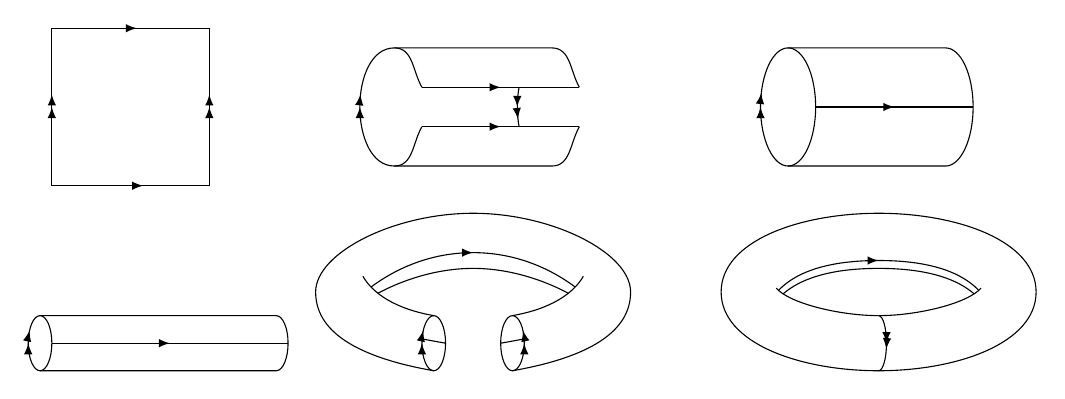
\begin{tikzpicture}
        \draw[postaction={decorate},decoration={
            markings,
            mark=at position .145 with {\arrow{latex}},
            mark=at position .375 with {\arrow{latex}},
            mark=at position .395 with {\arrow{latex}},
            mark=at position .615 with {\arrowreversed{latex}},
            mark=at position .855 with {\arrowreversed{latex}},
            mark=at position .875 with {\arrowreversed{latex}}}]
            (0,-1) -- +(2,0) -- +(2,2) -- +(0,2) -- cycle;
        \begin{scope}[xshift=4.7cm]
            \draw[postaction={decorate},decoration={
            markings,
            mark=at position .5 with {\arrow{latex}}}]
            (0,.25) -- ++(2,0);
            \draw[postaction={decorate},decoration={
            markings,
            mark=at position .5 with {\arrow{latex}}}]
            (0,-.25) -- ++(2,0);
            \draw[postaction={decorate},decoration={
            markings,
            mark=at position .5 with {\arrow{latex}},
            mark=at position .55 with {\arrow{latex}}}]
            (0,-.25) to[out=-120,in=0] (-.35,-.75) to[out=180,in=180] (-.35,.75) to[out=0,in=120] (0,.25);
            \draw (2,.25) to[out=120,in=0] (1.65,.75) -- (-.35,.75) (-.35,-.75) --  (1.65,-.75) to[out=0,in=-120] (2,-.25);
            \clip (0,.25) rectangle (2,-.25);
            \draw[postaction={decorate},decoration={
            markings,
            mark=at position .5 with {\arrow{latex}},
            mark=at position .58 with {\arrow{latex}}}]
            (1.65,.75) to[out=180,in=180] (1.65,-.75);
        \end{scope}
        \begin{scope}[xshift=9.7cm]
            \draw[postaction={decorate},decoration={
            markings,
            mark=at position .5 with {\arrow{latex}},}]
            (0,0) -- (2,0);
            \draw[postaction={decorate},decoration={
            markings,
            mark=at position .5 with {\arrow{latex}},
            mark=at position .55 with {\arrow{latex}}}]
            (0,0) arc[start angle=0,delta angle=-360,x radius=.35,y radius=.75];
            \draw (2,0) arc[start angle=0,delta angle=-90,x radius=.35,y radius=.75] -- ++(-2,0);
            \draw (2,0) arc[start angle=0,delta angle=90,x radius=.35,y radius=.75] -- ++(-2,0);
        \end{scope}
        \begin{scope}[yshift=-3cm]
            \draw[postaction={decorate},decoration={
            markings,
            mark=at position .5 with {\arrow{latex}},}]
            (0,0) -- (3,0);
            \draw[postaction={decorate},decoration={
            markings,
            mark=at position .5 with {\arrow{latex}},
            mark=at position .6 with {\arrow{latex}},}]
            (0,0) arc[start angle=0,delta angle=-360,x radius=.15,y radius=.35];
            \draw (3,0) arc[start angle=0,delta angle=-90,x radius=.15,y radius=.35] -- ++(-3,0);
            \draw (3,0) arc[start angle=0,delta angle=90,x radius=.15,y radius=.35] -- ++(-3,0);
        \end{scope}
        \begin{scope}[xshift=4cm,yshift=-3cm]
            \draw[postaction={decorate},decoration={
            markings,
            mark=at position .5 with {\arrow{latex}},
            mark=at position .6 with {\arrow{latex}},}]
            (1,0) arc[start angle=0,delta angle=-360,x radius=.15,y radius=.35];
            \draw (1,0) ++(-.15,-.35) .. controls +(170:1) and +(-90:.5) .. ++(-1.5,1) .. controls +(90:.5) and +(180:1) .. ++(2,1) .. controls +(0:1) and +(90:.5) .. ++(2,-1) .. controls +(-90:.5) and +(10:1) .. ++(-1.5,-1) coordinate (a);
            \draw[postaction={decorate},decoration={
            markings,
            mark=at position .5 with {\arrow{latex}},
            mark=at position .6 with {\arrow{latex}},}]
            (a) ++(-.15,.35) arc[start angle=0,delta angle=-360,x radius=-.15,y radius=.35];
            \draw (1,0) ++(-.15,.35) .. controls +(170:.5) and +(-60:.25) .. ++(-.9,.5) coordinate (b);
            \draw (a) ++(0,.7) .. controls +(10:.5) and +(240:.25) .. ++(.9,.5) coordinate (c);
        \end{scope}
        \begin{scope}[xshift=4cm,yshift=-3cm]
            \clip (1,0) ++(-.15,.35) .. controls +(170:.5) and +(-60:.25) .. ++(-.9,.5) -- ++(0,2) -| (c)  .. controls +(240:.25) and +(10:.5) .. ++(-.9,-.5);
            \draw (1,0) ++(-.15,-.35) ++(0,-.7) .. controls +(170:1) and +(-90:.5) .. ++(-1.5,.8) .. controls +(90:.5) and +(180:1) .. ++(2,1.2) .. controls +(0:1) and +(90:.5) .. ++(2,-1.2) .. controls +(-90:.5) and +(10:1) .. ++(-1.5,-.8);
            \draw[postaction={decorate},decoration={
            markings,
            mark=at position .5 with {\arrow{latex}},}]
            (1,0) ++(-.15,-.35) ++(0,-.8) .. controls +(170:1) and +(-90:.5) .. ++(-1.5,.8) .. controls +(90:.5) and +(180:1.2) .. ++(2,1.5) .. controls +(0:1.2) and +(90:.5) .. ++(2,-1.5) .. controls +(-90:.5) and +(10:1) .. ++(-1.5,-.8);
        \end{scope}
        \begin{scope}[xshift=4cm,yshift=-3cm]
        \clip  (a) ++(-.15,.35) arc[start angle=0,delta angle=-360,x radius=-.15,y radius=.35];
        \draw (a) ++(-.15,.35) .. controls +(10:1) and +(-90:.5) .. ++(1.5,.8);
        \end{scope}
        \begin{scope}[xshift=4cm,yshift=-3cm]
        \clip (1,0) arc[start angle=0,delta angle=-360,x radius=.15,y radius=.35];
        \draw (1,0) .. controls +(170:1) and +(-90:.5) .. ++(-1.5,.8);
        \end{scope}
        \begin{scope}[xshift=9cm,yshift=-3cm]
            \draw[postaction={decorate},decoration={
            markings,
            mark=at position .5 with {\arrow{latex}},
            mark=at position .6 with {\arrow{latex}},}]
            (1.5,.35) arc[start angle=90,end angle=-90,y radius=.35,x radius=.1];
            \draw (1.5,-.35) .. controls +(180:1) and +(-90:.65) .. ++(-2,1) .. controls +(90:.65) and +(180:1) .. ++(2,1) .. controls +(0:1) and +(90:.65) .. ++(2,-1) .. controls +(-90:.65) and +(0:1) .. ++(-2,-1); \draw (1.5,.35) .. controls +(180:.5) and +(-50:.25) .. ++(-1.3,.35) coordinate (b);
            \draw (1.5,.35) .. controls +(0:.5) and +(230:.25) .. ++(1.3,.35) coordinate (c);
        \end{scope}
        \begin{scope}[xshift=9cm,yshift=-3cm]
            \clip (1.5,.35) .. controls +(180:.5) and +(-50:.25) .. ++(-1.3,.35) -- ++(0,2) -| (c)  .. controls +(230:.25) and +(0:.5) .. ++(-1.3,-.35);
            \draw (1.5,-.35) ++(0,-.7) .. controls +(180:1) and +(-90:.65) .. ++(-1.5,1) .. controls +(90:.65) and +(180:1) .. ++(1.5,1) .. controls +(0:1) and +(90:.65) .. ++(1.5,-1) .. controls +(-90:.65) and +(0:1) .. ++(-1.5,-1);
            \draw[postaction={decorate},decoration={
            markings,
            mark=at position .5 with {\arrow{latex}},}]
            (1.5,-.35) ++(0,-.6) .. controls +(180:1) and +(-90:.65) .. ++(-1.5,1) .. controls +(90:.65) and +(180:1) .. ++(1.5,1) .. controls +(0:1) and +(90:.65) .. ++(1.5,-1) .. controls +(-90:.65) and +(0:1) .. ++(-1.5,-1);
        \end{scope}
    \end{tikzpicture}
    \caption[Surgery Theory - Plane Representation of a Torus]{The unit square with a particular equivalence relation on it can be used to represent a torus.}
    \label{fig:surgery_theory_plane_representation_of_a_torus}
\end{figure}
\begin{theorem}
There exist manifolds $X$ and $Y$ such that $\dim(X) = \dim(Y)$, $X\simeq Y$, yet $X$ and $Y$ are not homeomorphic.
\end{theorem}
\begin{proof}
For let $X = S^{2}\setminus\{(0,0,1),(0,1,0),(1,0,0)\}$, and let $Y = T^{2}\setminus\{(1,0,0)\}$. That is, $X$ is a sphere with three points removed, and $Y$ is a torus with one point removed. Then $\dim(X) = \dim(Y) = 2$. Moreover, $X\simeq Y$. For $X$ is homeomorphic to the plane with $2$ points removed. This is homotopy equivalent to a figure $8$. Using the square representation of a torus in Fig.~\ref{fig:surgery_theory_plane_representation_of_a_torus} we see that the torus with a point removed is also homotopy equivalent to a figure $8$. But homotopy equivalence is an equivalence relation, and thus $X\simeq Y$. But the a sphere is not homeomorphic to a torus, and similarly a sphere with $3$ points removed is not homeomorphic to a torus with $1$ point removed.
\end{proof}
Fig.~\ref{fig:surgery_theory_homotopy_equivalence_sphere_with_3_holes_torus_with_1_hole} shows how both $S^{2}$ with three points removed and $T^{2}$ with one point removed are homotopy equivalent. Recall that $\mathbb{R}^{2}\setminus \{(0,0)\}$ is homotopy equivalent to $S^{1}$. In a similar manner, the plane with two points removed is homotopy equivalent to two circles whose intersection contains a single points (That is, a figure-$8$). While the ``Proof," given was hand wavy, the fact that the sphere is not homeomorphic to the torus comes from the fact that these two objects have different boundary components, something preserved by homeomorphism. Intiutively, one can think of removing a great circle (Or a ``line") from the sphere. Removing such an object creates two disconnected components. However, removing a circle from the torus still leaves one connected surface. The next question is ``What about compact manifolds without boundary?"
\begin{theorem}[The Generalized Poincare-Conjecture]
If $X$ is an $n$ dimensional manifold that is homotopy equivalent to $S^{n}$, then $X$ is homeomorphic to $S^{n}$.
\end{theorem}
\begin{definition}
A rigid manifold is a manifold $X$ such that for all homotopy equivalent closed manifolds $Y$, $X$ is homeomorphic to $Y$.
\end{definition}
\begin{figure}[H]
    \centering
    \resizebox{!}{0.3\textheight}{
    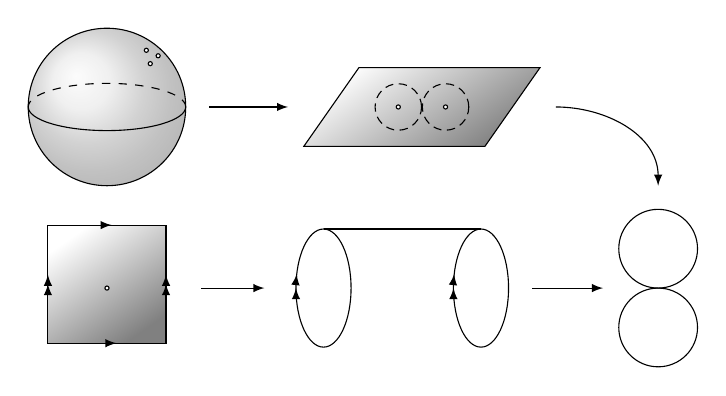
\begin{tikzpicture}
        \shade[ball color = gray!40, opacity = 0.4] (0,0) circle (1cm);
        \draw (0,0) circle (1cm);
        \draw (-1,0) arc (180:360:1 and 0.3);
        \draw[dashed] (1,0) arc (0:180:1 and 0.3);
        \fill[fill=white,draw=black] (0.55,0.55) circle (0.75pt);
        \fill[fill=white,draw=black] (0.65,0.65) circle (0.75pt);
        \fill[fill=white,draw=black] (0.5,0.72)  circle (0.75pt);
        \draw[>=latex,draw=black,->] (1.3cm,0) -- (2.3cm,0);
        \shade[fill = gray,shading angle = 215](2.5cm,-0.5cm) -- (3.2cm, 0.5cm) -- (5.5cm,0.5cm) -- (4.8cm,-0.5cm) -- cycle;
        \draw (2.5cm,-0.5cm) -- (3.2cm, 0.5cm) -- (5.5cm,0.5cm) -- (4.8cm,-0.5cm) -- cycle;
        \draw[draw=black,densely dashed] (3.7cm,0) circle (0.295cm);
        \draw[draw=black,densely dashed] (4.3cm,0) circle (0.295cm);
        \fill[fill=white,draw=black] (3.7cm,0) circle (0.75pt);
        \fill[fill=white,draw=black] (4.3cm,0) circle (0.75pt);
        \draw[>=latex,draw=black,->] (5.7cm,0) to [in=90, out=0] (7cm,-1cm);
        \draw[>=latex,draw=black,->] (1.2cm,-2.3cm) -- (2cm,-2.3cm);
        \shade[fill = gray,shading angle = 215](-0.75,-3cm) -- +(1.5cm,0) -- +(1.5cm,1.5cm) -- +(0,1.5cm) -- cycle;
        \fill[fill=white,draw=black] (0,-2.3cm) circle (0.75pt);
        \draw[postaction={decorate},decoration={
            markings,
            mark=at position .145 with {\arrow{latex}},
            mark=at position .375 with {\arrow{latex}},
            mark=at position .395 with {\arrow{latex}},
            mark=at position .615 with {\arrowreversed{latex}},
            mark=at position .855 with {\arrowreversed{latex}},
            mark=at position .875 with {\arrowreversed{latex}}}]
        (-0.75,-3cm) -- +(1.5cm,0) -- +(1.5cm,1.5cm) -- +(0,1.5cm) -- cycle;
        \draw[postaction={decorate},decoration={
            markings,
            mark=at position .5 with {\arrow{latex}},
            mark=at position .55 with {\arrow{latex}}}]
            (3.1cm,-2.3cm) arc[start angle=0,delta angle=-360,x radius=.35,y radius=.75];
            \draw (2.75cm,-1.55cm) -- ++(2cm,0);
            \draw[postaction={decorate},decoration={
            markings,
            mark=at position .5 with {\arrow{latex}},
            mark=at position .55 with {\arrow{latex}}}]
            (5.1cm,-2.3cm) arc[start angle=0,delta angle=-360,x radius=.35,y radius=.75];
        \draw[>=latex,draw=black,->] (5.4cm,-2.3cm) -- (6.3cm,-2.3cm);
        \draw[draw = black] (7cm,-1.8cm) circle (0.5cm);
        \draw[draw = black] (7cm,-2.8cm) circle (0.5cm);
    \end{tikzpicture}}
    \caption{Caption}
    \label{fig:surgery_theory_homotopy_equivalence_sphere_with_3_holes_torus_with_1_hole}
\end{figure}
The question then becomes ``Which manifolds are rigid, and which are not?" From the Poincare theorem, $S^{n}$ is rigid for all $n\in \mathbb{N}$. The first example of a non-rigid manifold came in the 1930's from Franz, Reidemeister, and de Rham, and is called a Lens Space. Let $p$ and $q$ be coprime positive integers. Divide $S^{3}$ into $p$ equal parts, and then divide this into its northern and southern hemispheres. Take a piece of the northern hemisphere and move it over $q$ pieces, and then glue this to the southern hemisphere. Take the piece that is already there and move it over $q$ pieces, and then glue that to the northern hemisphere. Repeat this process until all slices are done. The is called the Lens Space $L(p,q)$. $L(1,1)$ is simply the sphere. $L(2,1)$ is the real projective plane $\mathbb{RP}^{2}$. See Fig.~\ref{fig:surgery_theory_lens_space_drawing} to see how this construction occurs. It can be shown that for distinct pairs $(p,q), (p',q')$, that $L(p,q)$ is homotopy equivalent to $L(p',q')$, but not homeomorphic.
\begin{figure}[H]
    \centering
    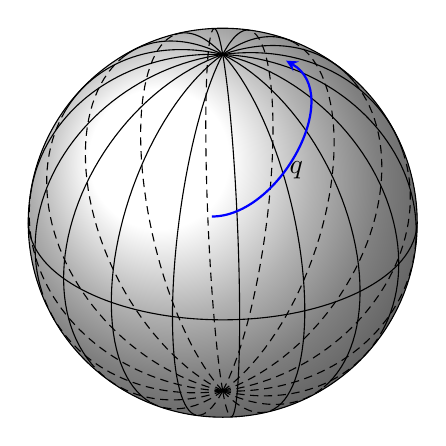
\begin{tikzpicture}
    \pgfplotsset{compat=1.9}
        \def\tilt{45}
        \def\azimuth{30}
        \begin{axis}[%
        axis equal,
        width=14cm,
        height=14cm,
        hide axis,
        enlargelimits=0.3,
        view/h=\tilt,
        view/v=\azimuth,
        scale uniformly strategy=units only,
        colormap={bluewhite}{color=(blue) color=(white)}]
        \coordinate (X) at (axis cs: 1,0,0);
        \coordinate (-X) at (axis cs: -1,0,0);
        \coordinate (Y) at (axis cs: 0,1,0);
        \coordinate (-Y) at (axis cs: 0,-1,0);
        \coordinate (Z) at (axis cs: 0,0,1);
        \coordinate (-Z) at (axis cs: 0,0,-1);
        \filldraw[ball color=white] (axis cs: 0,0,0) circle (2.47cm);
        \pgfplotsinvokeforeach {0}{
        \pgfplotsextra{ 
        \pgfmathsetmacro\sinVis{sin(#1)/cos(#1)*sin(\azimuth)/cos(\azimuth)}
         % angle of "visibility"
        \pgfmathsetmacro\angVis{asin(min(1,max(\sinVis,-1)))}
        \coordinate (X) at (axis cs: {cos(#1)},0,{sin(#1)});
        \draw (X) arc (0:\tilt+\angVis:{100*cos(#1)}) (X) arc (0:-180+\tilt-\angVis:{100*cos(#1)});}}
        \foreach \a in {0,20,...,359}
        {\pgfmathsetmacro{\Bound}{-60*cos(\a+45)}
        \addplot3[domain=\Bound:90, samples=45,samples y=0] ({cos(\a)*cos(x)},{sin(\a)*cos(x)},{sin(x)});
        \addplot3[domain=-90:\Bound, samples=45,samples y=0, densely dashed] ({cos(\a)*cos(x)},{sin(\a)*cos(x)},{sin(x)});}
        \draw[draw=blue,>={stealth[blue]},->,thick] (3.2cm,3.5cm,3.5cm) to [in = 330, out=0] node [below] {$q$} (2.0cm,6.6cm,5cm);
        \end{axis}
    \end{tikzpicture}
    \caption{How to construct $L(p,q)$.}
    \label{fig:surgery_theory_lens_space_drawing}
\end{figure}
We move on to the structure set of topological spaces, in particular closed topological manifolds $\mathcal{M}$.
\begin{definition}
A manifold structure on a closed manifold $X$ of dimension $n$ is a homotopy equivalence between $X$ and a closed manifold $N$ of dimension $n$, $f:N\rightarrow X$, $g:X\rightarrow N$.
\end{definition}
\begin{definition}
Equivalent manifold structures are manifold structures $f:N_{1}\rightarrow X$, $g:N_{2}\rightarrow X$ such that there is a homeomorphism $h:N\rightarrow M$ such that $f$ is homotopic to $g\circ h$.
\end{definition}
The equivalent classes of $Y$ is called the structure set of $Y$. This set contains maps like $f_{1},f_{2}$. If $g$ is a homeomorphism, then $f_{1} = f_{2}$.
\begin{example}
$S^{Top}(S^{n}) = \{S^{n}\}$
\end{example}
If $|S(Y)|>1$, then $Y$ is non-rigid.
\begin{example}
$|S(L(p,q))| \ne 1$
\end{example}
A few questions naturally arise from the definition of the structure set:
\begin{enumerate}
\begin{multicols}{2}
    \item Is $S^{Top}(Y)$ a group?
    \begin{itemize}
        \item Sometimes.
    \end{itemize}
    \item Is $^{Top}S(Y)$ fininte?
    \begin{itemize}
        \item Sometimes.
        \begin{itemize}
            \item $|S^{Top}(S^{n})| = 1$
            \item $|S^{Top}(T^{n})| = 2^{n}$
        \end{itemize}
    \end{itemize}
    \item Can $S(Y)$ be infinite?
    \begin{itemize}
        \item Yes.
        \begin{itemize}
            \item $|S^{Top}(\mathbb{RP}^{5})|$ - Finite.
            \item $|S^{Top}(\mathbb{RP}^{6})|$ - Finite.
            \item $|S^{Top}(\mathbb{RP}^{7})|$ - \underline{Infinite}.
            \item $|S^{Top}(\mathbb{RP}^{8})|$ - Finite.
        \end{itemize}
    \end{itemize}
\end{multicols}
\end{enumerate}
A review of some concepts from algebraic topology.
\begin{definition}
A path in a topological space $X$ is a continuous function $f:I\rightarrow X$
\end{definition}
\begin{definition}
A loop in a topological space $X$ is a path $f$ such that $f(0)=f(1)$.
\end{definition}
\begin{definition}
The fundamental group of a topological space $X$ is the set $\pi_{1}(X) = \{f\in C(I,X):f(0) = f(1)\}/h$, where $h$ is the modulo of homotopy, equipped with the concatenation operation:
\begin{equation*}
    (f*g)(t) = \begin{cases} f(2t), & 0\leq t < \frac{1}{2}\\ g(2t-1), & \frac{1}{2}\leq t < 1\end{cases}
\end{equation*}
\end{definition}
\begin{example}
\begin{align*}
    \begin{rcases*} \pi_{1}(S^{n}) = \{e\}\\ \pi_{1}(T^{n}) = \mathbb{Z}^{n} \end{rcases*} \textrm{No Torsion}\\
    \begin{rcases*} \pi_{1}(\mathbb{RP}^{n}) = \mathbb{Z}_{2} \\ \pi_{1}(L(p,q)) = \mathbb{Z}_{p} \end{rcases*} \textrm{Torsion}
\end{align*}
\end{example}
\begin{definition}
The order of an element $g$ of a group $G$ is $o(g) = \inf\{n\in \mathbb{N}:a^{n} = e\}$.
\end{definition}
\begin{definition}
A group with torsion is a group $G$ such that there exists $g\in G$ such that $g\ne e$ and $1<o(g)<\infty)$.
\end{definition}
\begin{definition}
A torsion group is a group $G$ such that for all $g\in G$ such that $g\ne e$, $o(g)<\infty$.
\end{definition}
We now arrive at the first ``Surgery Theory" based theorem.
\begin{theorem}
If $n\geq 5$, $n\equiv 3\! \mod 4$, and $\pi_{1}(X)$ is a torsion group, then $|S^{Top}(X^{n})| = \infty$, and $\pi_{1}(X)$ has torsion.
\end{theorem}
Some other gems: $S^{Top}(\mathbb{CP}^{2}) = \mathbb{Z}_{2}$. Chern Manifolds are a thing.
\subsubsection{The Unsolvable Word Problem}
\begin{definition}
A presentation of a group $G$ is a set $H\subset G$ of generators and a set $R$ of relations on $H$. This is denoted $G = \langle H|R\rangle$.
\end{definition}
\begin{example}
\
\begin{enumerate}
    \item $\langle a | a^{n} = e\rangle$ is the cyclic group of order $n$ generated by $a$.
    \item $\langle g,h|hg = gh\rangle = \mathbb{Z}^{2}$
    \item $\langle g,h|g^{n} = e, h^{2} = e\rangle = \mathbb{Z}_{2}*\mathbb{Z}_{n}$
    \item $\langle g,h|g^{n} = e,h^{2} = e, gh=h^{-1}g\rangle = D_{2n}$
\end{enumerate}
\end{example}
\begin{remark}
The word problem on unsolvability: Given two group presentations, there is no algorithm to show that they are isomorphic.
\end{remark}
\begin{definition}
A finitely presented group is a group with a presentation $\langle H|R\rangle$ such that $H$ and $R$ are finite.
\end{definition}
\begin{theorem}
If $n\geq 5$ and $G$ is finitely presented, then there is a closed $n$ dimensional manifold $\mathcal{M}$ such that $\pi_{1}(\mathcal{M}) = G$.
\end{theorem}
\subsubsection{Exact Sequences and Surgery Exact Sequences}
\begin{definition}
An exact sequence $\cdots G_{3}\overset{f_{3}}{\rightarrow}G_{2}\overset{f_{2}}{\rightarrow}G_{1}\overset{f_{1}}{\rightarrow}G_{0}$ is a sequence $f_{n}$ of homomorphisms and a sequence $G_{n}$ of groups such that $\Im(f_{n+1}) = \ker(f_{n})$
\end{definition}
\begin{remark}
Note, the definition requires that the $f_{n}$ are \textit{homomorphisms}, not homeomorphisms. Homeomorphism is a topological notion, not an algebraic one.
\end{remark}
\begin{example}
$0\overset{f}{\rightarrow}G\overset{g}{\rightarrow}H$. $\Im(f) = 0$, $\ker(g) = 0$. So $g$ is injective.
\end{example}
\begin{example}
$G\overset{f}{\rightarrow}H\overset{g}{\rightarrow}0$, $\ker(g) = H$, $\Im(f) = H$, $f$ is surjective.
\end{example}
\begin{definition}
A short exact sequence is an exact sequence $0\overset{f}{\rightarrow}G\overset{g}{\rightarrow}H\overset{h}{\rightarrow}L\overset{f_{3}}{\rightarrow}0$
\end{definition}
We have, from the previous examples, than in an exact sequence $f$ must be injective and $g$ must be surjective. We now move onto surgery exact sequences (See Wall et. al). Let $n\geq 5$, and $\mathcal{M}$ be a closed manifold of dimension $n$. Let $\pi = \pi_{1}(\mathcal{M})$. Let Cat have the following meaning:
\begin{itemize}
    \item Top: Category of continuous maps. That is, the topological catagory.
    \item PL: Piece-Wise linear category. Maps are piece-wise linear.
    \item Diff: Differentiable category. Maps are diffeomorphisms.
\end{itemize}
\begin{example}
\
\begin{enumerate}
    \begin{multicols}{2}
        \item $S^{Top}(S^{n}) = \{S^{n}\}$
        \item $S^{PL}(S^{n}) = \{S^{n}\}$
        \item $|S^{Diff}(S^{7})| = 28$ (Milnor)
        \item $|S^{PL}(T^{n})| = 2^{n}$ - Non-Rigid.
    \end{multicols}
\end{enumerate}
\end{example}
A surgery exact sequence is a sequence of the form:
\begin{align*}
    S^{Cat}(\mathcal{M}\times S^{1}) \rightarrow [\mathcal{M}\times S^{1},F/Cat] &\rightarrow L_{n+1}(\pi_{1}(\mathcal{M})) \rightarrow S^{Cat}(\mathcal{M}) \rightarrow \cdots\\
    \cdots &\rightarrow [\mathcal{M},F/Cat] \rightarrow L_{n}(\pi_{1}(\mathcal{M}))
\end{align*}
Here, $L_{n}(\pi_{1}(M))$ is a \textit{Wall Group}, and $[A,B]$ is the notation for the collection of homotopy classes of maps between $A$ and $B$.
\subsection{Lecture 2: Surgery Structure Sets}
\begin{wrapfigure}[6]{r}{0.2\textwidth}
\vspace{-6ex}
\centering
\begin{tikzcd}[row sep=small,column sep=large]
N_{1} \arrow[dd,"g"] \arrow[dr, "f_{1}"] \\
& M \\
N_{2} \arrow[ur, "f_{2}" below]
\end{tikzcd}
\caption[Surgery Theory Commutative Diagram]{Commutative Diagram for $g$}
\label{fig:wellesley_surgery_theory_commutative_diagram_for_g_for_two_homotopy_equivalences}
\end{wrapfigure}
Let $X,M_{1}$, and $M_{2}$ be closed, compact $n$-dimensional manifolds without boundary. Two homotopy equivalences $f_{i}:M_{i}\rightarrow X$ are called equivalent if there exists a cobordism $(W;M_{1},M_{2})$ and a map $(F;f_{1},f_{2}):(W;M_{1},M_{2})\rightarrow (X\times [0,1];X\times \{0\},X\times\{1\})$ such that $F,f_{1},f_{2}$ are homotopy equivalences. The structure set $S(X)$ is the set of equivalence classes of homotopy equivalences $f:M\rightarrow X$ from closed manifolds of dimension $n$ to $X$.\hfill
\begin{definition}
The surgery structure set of a closed (without boundary) compact manifold $M$ is $S(M) = \{f:N^{n}\rightarrow M^{n}|f\textrm{ is a Homotopy Equivalence}\}$
\end{definition}
\begin{definition}
The base point of a surgery structure set is the map $id_{X}:X\rightarrow X$.
\end{definition}
Let $N_{1}$ and $N_{2}$ be two manifold structures. And let $f_{1}:N_{1}^{n}\rightarrow M^{n}$ and $f_{2}:N_{2}^{n}\rightarrow M^{n}$ be two homotopy equivalences. We call $g:N_{1}\rightarrow N_{2}$ a cat-homeomorphism if $g$, together with $f_{1}$ and $f_{2}$, form the commutative diagram in figure \ref{fig:wellesley_surgery_theory_commutative_diagram_for_g_for_two_homotopy_equivalences}. That is, $g$ is a cat-homeomorphism if it homotopoy commutes.
\begin{remark}
Cat means category. There are three types: Top, PL, and Diff. 
    \begin{itemize}
        \begin{multicols}{3}
            \item Top: Topological
            \item PL: Piece-wise Linear
            \item Diff: Diffeomorphism
        \end{multicols}
    \end{itemize}
\end{remark}
\begin{example}
Some examples of surgery structure sets:
    \begin{enumerate}
        \begin{multicols}{3}
            \item $S^{Top}(S^{n})=\{S^{n}\}$
            \item $S^{PL}(S^{n}) = \{S^{n}\}$
            \item $S^{Diff}(S^{7}) = \mathbb{Z}_{28}$
        \end{multicols}
    \end{enumerate}
\end{example}
\subsubsection{Orientable and Non-Orientable}
Stiefel-Whitney classes $w_{1},\hdots, w_{n}$ are cohomological classes. Orientiable means that $w_{1} = 0$.
\begin{example}
\
\begin{enumerate}
    \begin{multicols}{2}
    \item $\mathbb{RP}^{2}$ - Non-Orientable
    \item $\mathbb{RP}^{4}$ - Non-Orientable
    \item $\mathbb{RP}^{6}$ - Non-Orientable
    \item $\mathbb{RP}^{8}$ - Non-Orientable
    \item $\mathbb{RP}^{3}$ - Orientable
    \item $\mathbb{RP}^{5}$ - Orientable
    \item $\mathbb{RP}^{7}$ - Orientable
    \item $\mathbb{CP}^{n}$ - Orientable for all $n\in\mathbb{N}$
    \end{multicols}
\end{enumerate}
\end{example}
Returning to surgery exact sequences, the goal is to compute $S^{Cat}(\mathcal{M}^{n})$, where $n$ is the dimension of $\mathcal{M}^{n}$. The notion of a surgery helps solve this question. Let $X = \mathbb{S}^{2}\setminus\{(a_{1},b_{1},c_{1}),(a_{2},b_{2},c_{2})\}$. That is, the sphere with two points removed. Stretch these two points out to create a sphere with two holes removed. One could imagine taking a hollow cylinder and stretching it to connect the two holes in the sphere. The result is a spherical coffee cup, as shown in Fig.~\ref{fig:surgery_theory_example_of_a_surgery}. This figure can be continuously deformed into a torus.
\begin{figure}[H]
    \centering
    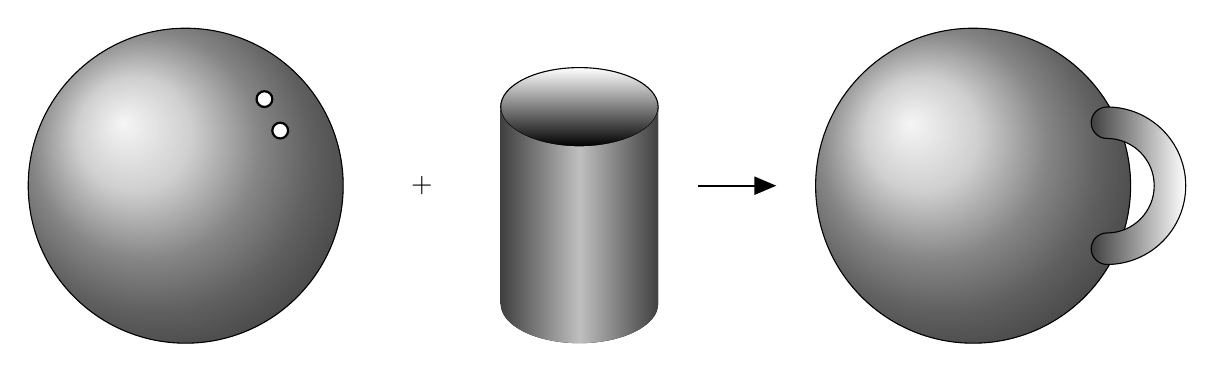
\begin{tikzpicture}
        \fill[ball color = gray!50!white,draw=black] (0,0) circle (2);
        \fill[fill=white,draw=black,thick] (1,1.1) circle (0.1);
        \fill[fill=white,draw=black,thick] (1.2,0.7) circle (0.1);
        \node at (3,0) {$+$};
        \fill[bottom color = black,top color = white,draw=black] (5,1) ellipse (1 and 0.5);
        \fill[left color=gray!50!black,right color=gray!50!black,middle color=gray!50,shading=axis] (4,1) -- (4,-1.5) arc(180:360:1 and 0.5) -- (6,1) arc(360:180:1 and 0.5);
        \draw[draw=black,thick,>=triangle 45,->] (6.5,0) -- (7.5,0);
        \fill[ball color = gray!50!white,draw=black] (10,0) circle (2);
        \fill[left color=black!50!gray,right color=white,draw=black,thin] (11.7,1) arc(90:-90:1) arc(-90:-270:0.2) arc(-90:90:0.6) arc(-90:-270:0.2);
    \end{tikzpicture}
    \caption{A zero surgery on the sphere.}
    \label{fig:surgery_theory_example_of_a_surgery}
\end{figure}
Recall that $S^{0}$ is two points, and that $D^{2}$ is the open unit disc. Then $S^{0}\times D^{2}$ is simply two disjoint open unit discs. This is a good representation of the idea of the disjoint union, denoted $X\coprod Y$. We have that:
\begin{equation*}
    S^{0}\times D^{2} = D^{2} \coprod D^{2}
\end{equation*}
We can also represent a cylinder as the closed $S^{1}\times \overline{D}^{1}$. The codimension of a surgery is the dimension of the object minus the dimension of a surgery. So, for the surgery in Fig.~\ref{fig:surgery_theory_example_of_a_surgery}, the dimension of the entire thing is $2$, the dimension of the surgery is $2$, so the codimension is $0$. This is called a Zero-Surgery. A zero-surgery takes out $2$ holes and connects them with a tube.
\begin{figure}[H]
    \centering
    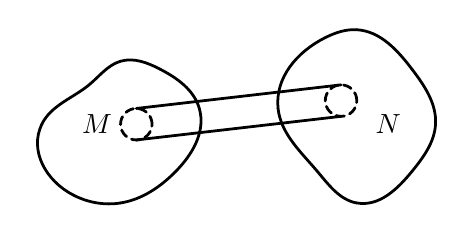
\begin{tikzpicture}[line width=1pt,line cap = round,>={Stealth[black]},every edge/.style={draw=black,very thick}]
        \node[fill=black,circle,inner sep=0pt,outer sep=0pt] at (0,0) (a) {};
        \node[fill=black,circle,inner sep=0pt,outer sep=0pt] at (-0.6,0.1) (b) {};
        \node[fill=black,circle,inner sep=0pt,outer sep=0pt] at (-1,1) (c) {};
        \node[fill=black,circle,inner sep=0pt,outer sep=0pt] at (-0.4,1.5) (d) {};
        \node[fill=black,circle,inner sep=0pt,outer sep=0pt] at (0, 1.8) (e) {};
        \node[fill=black,circle,inner sep=0pt,outer sep=0pt] at (0.5, 1.7) (f) {};
        \node[fill=black,circle,inner sep=0pt,outer sep=0pt] at (1,1.2) (g) {};
        \node[fill=black,circle,inner sep=0pt,outer sep=0pt] at (0.7,0.4) (h) {};
        \node at (-0.3,1) (i) {$M$};
        \path[draw,use Hobby shortcut,closed=true](a) .. (b) .. (c) .. (d) .. (e) .. (f) .. (g) .. (h);
        \node[fill=black,circle,inner sep=0pt,outer sep=0pt] at (3,0) (a1) {};
        \node[fill=black,circle,inner sep=0pt,outer sep=0pt] at (2.5,0.4) (b1) {};
        \node[fill=black,circle,inner sep=0pt,outer sep=0pt] at (2,1.2) (c1) {};
        \node[fill=black,circle,inner sep=0pt,outer sep=0pt] at (2.6,2.1) (d1) {};
        \node[fill=black,circle,inner sep=0pt,outer sep=0pt] at (3, 2.2) (e1) {};
        \node[fill=black,circle,inner sep=0pt,outer sep=0pt] at (3.7, 1.7) (f1) {};
        \node[fill=black,circle,inner sep=0pt,outer sep=0pt] at (4,1) (g1) {};
        \node[fill=black,circle,inner sep=0pt,outer sep=0pt] at (3.7,0.4) (h1) {};
        \node at (3.4,1) (i1) {$N$};
        \draw[draw=black,densely dashed] (0.2,1) circle (0.2);
        \draw[draw=black,densely dashed] (2.8,1.3) circle (0.2);
        \draw (0.2,1.2) -- (2.8,1.5);
        \draw (0.2,0.8) -- (2.8,1.1);
        \path[draw,use Hobby shortcut,closed=true](a1) .. (b1) .. (c1) .. (d1) .. (e1) .. (f1) .. (g1) .. (h1);
    \end{tikzpicture}
    \caption[Surgery Theory - A Zero Surgery]{A Zero Surgery between $N$ and $M$.}
    \label{fig:surgery_theory_a_zero_surgery}
\end{figure}
Let $\mathcal{M}^{n}$ be an $n$ dimensional manifold. Embed $S^{k}\times D^{n-k}$ into $\mathcal{M}^{n}$. Then $\partial(S^{k}\times D^{n-k}) = S^{k}\times S^{n-k-1}$, where $\partial(X)$ is the boundary of $X$. Remove $\partial(S^{k}\times D^{n-k})$ and glue $S^{k+1}D^{n-k-1}$. Note that $\dim(S^{k+1}\times D^{n-k-1}) = \dim(S^{k}\times D^{n-k}) = n$. We alse have that $\partial(D^{k+1}\times S^{n-k-1}) = S^{k}\times S^{n-k-1}$. Glue $\mathcal{M}^{n}\cup (D^{k+1}\times S^{n-k-1})$ along $\partial(S^{k}\times S^{n-k-1})$.
\begin{figure}[H]
    \centering
    \resizebox{!}{0.2\textheight}{
    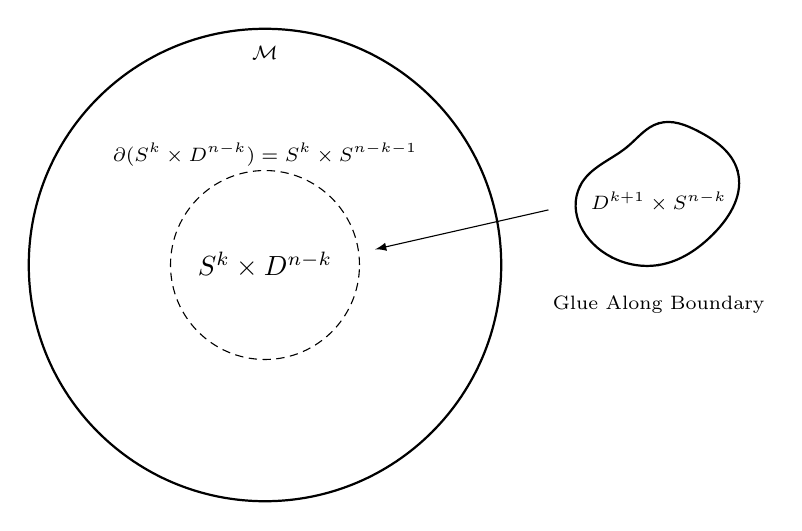
\begin{tikzpicture}
        \draw[draw=black,densely dashed] (0,0) circle (1.2);
        \draw[draw=black,thick] (0,0) circle (3);
        \node at (0,2.7) {\scriptsize{$\mathcal{M}$}};
        \node at (0,0) {$S^{k}\times D^{n-k}$};
        \node at (0,1.4) {\scriptsize{$\partial(S^{k}\times D^{n-k}) = S^{k}\times S^{n-k-1}$}};
        \node[fill=black,circle,inner sep=0pt,outer sep=0pt] at (5,0) (a) {};
        \node[fill=black,circle,inner sep=0pt,outer sep=0pt] at (4.4,0.1) (b) {};
        \node[fill=black,circle,inner sep=0pt,outer sep=0pt] at (4,1) (c) {};
        \node[fill=black,circle,inner sep=0pt,outer sep=0pt] at (4.6,1.5) (d) {};
        \node[fill=black,circle,inner sep=0pt,outer sep=0pt] at (5, 1.8) (e) {};
        \node[fill=black,circle,inner sep=0pt,outer sep=0pt] at (5.5, 1.7) (f) {};
        \node[fill=black,circle,inner sep=0pt,outer sep=0pt] at (6,1.2) (g) {};
        \node[fill=black,circle,inner sep=0pt,outer sep=0pt] at (5.7,0.4) (h) {};
        \node at (5,0.8) {\scriptsize{$D^{k+1}\times S^{n-k}$}};
        \draw[>=latex,draw=black,->] (3.6,0.7) -- (1.4,0.2);
        \node at (5,-0.5) {\scriptsize{Glue Along Boundary}};
        \path[draw,use Hobby shortcut,closed=true,thick](a) .. (b) .. (c) .. (d) .. (e) .. (f) .. (g) .. (h);
    \end{tikzpicture}}
    \caption[Surgery Theory - Surgery Example]{Gluing $D^{k+1}\times S^{n-k}$ along $\partial(S^{k}\times D^{n-k})$. The new manifold is $\mathcal{M}^{n}\setminus (S^{k}\times D^{n-k}\coprod (D^{k+1}\times S^{n-k-1})$}
    \label{fig:surgery_theory_glueing_S_k_D_n_k_to_M}
\end{figure}
We now consider $k$ surgeries $\mathcal{M}\overset{\textrm{k-surgery}}{\longrightarrow}\mathcal{N}$.  We have seen $S^{2}\overset{\textrm{0-surgery}}{\longrightarrow} T^{2}$. Note: $\pi_{1}(S^{2})$ is trivial, and $\pi_{1}(T^{2}) = \mathbb{Z}^{2}$. This happens because $n<5$. When $n\geq 5$, we have the following result.
\begin{theorem}
If $\mathcal{M}$ is an $n$ dimensional manifold, $n\geq 5$, and if $\mathcal{N}$ is the result of a $k$ surgery on $\mathcal{M}$, then $\pi_{1}(\mathcal{M}) = \pi_{1}(\mathcal{N})$.
\end{theorem}
\subsubsection{More On Surgery Exact Sequences}
Recall that a surgery exact sequence looks like the following:
\begin{equation*}
    \underset{\textrm{Group}}{\underbrace{L_{n+1}(\mathbb{Z}\pi_{1}\mathcal{M})}} \rightarrow \cdots \rightarrow \underset{\textrm{Maybe a Group}}{\underbrace{S^{Cat}(\mathcal{M}^{n})}} \rightarrow \underset{\textrm{Group}}{\underbrace{[M,F/O]}} \rightarrow \underset{\textrm{Group}}{\underbrace{L_{n}(\mathbb{Z}\pi_{1}(\mathcal{M}))}} 
\end{equation*}
An exact sequence of groups is of then form $G_{n+1}\overset{g_{n}}{\rightarrow} G_{n}\rightarrow \hdots$, where $\Im(g_n) = \ker(g_{n-1})$. We broaden our notion of exactness:
\begin{equation*}
    \cdots \rightarrow L_{n+1}(\mathbb{Z}\pi_{1}(\mathcal{M})) \dashrightarrow S^{Cat}(\mathcal{M}) \overset{g}{\rightarrow} [\mathcal{M},F/O] \overset{\sigma}{\rightarrow} L_{n}(\mathbb{Z}\pi_{1}(\mathcal{M}))
\end{equation*}
The dotted line means $L_{n+1}(\mathbb{Z}\pi_{1}(\mathcal{M}))$ acts on $S^{Cat}(\mathcal{M})$. Exact means that $\Im(g) = \ker(\sigma)$. Each element $f\in [M,F/O]$ either pulls back to $\emptyset$ or something non-empty. If non-empty, you get a blob in $S^{Cat}(\mathcal{M})$: $f^{-1}(\{x\})$. But:
\begin{equation*}
    \underset{f\in [M,F/O]}{\cup}g^{-1}(\{f\}) = S^{Cat}(\mathcal{M})
\end{equation*}
This process creates a partition of $S^{Cat}(\mathcal{M})$. Now, $L_{n+1}(\mathbb{Z}(\pi_{1}\mathcal{M}))$ acts on $S^{Cat}(\mathcal{M})$ in some fashion. Partition the space into orbits. Exactness here means that partitioning by point inverses is the same as partitioning by orbits. That is, the two partitions are identical. See Fig.~\ref{fig:surgery_theory_partition_of_S_Cat} for a partioning into orbits.
\begin{figure}[H]
    \centering
    \resizebox{!}{0.15\textheight}{
    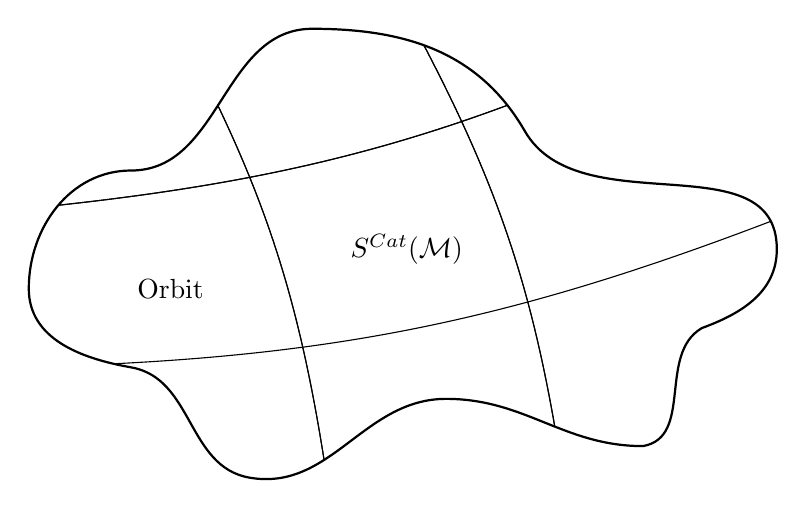
\begin{tikzpicture}
        \path coordinate (aux0) at (0,1.5) coordinate (aux1) at (0,3.5) coordinate (aux2) at (10,3.5) coordinate (aux3) at (9,6) coordinate (aux4) at (4,0) coordinate (aux5) at (7,0) coordinate (aux6) at (2,6) coordinate (aux7) at (5,6) coordinate (esp1) at (0.2,2.5) coordinate (esp2) at (1.5,1.5) coordinate (esp3) at (3,0.1) coordinate (esp4) at (5.5,1.1) coordinate (esp5) at (8,0.5) coordinate (esp6) at (8.75,2) coordinate (esp7) at (9.7,3) coordinate (esp8) at (6.5,4.5) coordinate (esp9) at (3.8,5.8) coordinate (esp10) at (1.5,4);
        \draw[line width=0.8pt] (esp1) to[out=-90,in=170] (esp2) to[out=-10,in=170] (esp3) to[out=-10,in=180] (esp4) to[out=0,in=180] (esp5) to[out=10,in=-150] (esp6) to[out=20,in=-90] (esp7) to[out=90,in=-60] (esp8) to[out=120,in=0] (esp9) to[out=180,in=0] (esp10) to[out=180,in=90] cycle;    
        \clip (esp1) to[out=-90,in=170] (esp2) to[out=-10,in=170] (esp3) to[out=-10,in=180] (esp4) to[out=0,in=180] (esp5) to[out=10,in=-150] (esp6) to[out=20,in=-90] (esp7) to[out=90,in=-60] (esp8) to[out=120,in=0] (esp9) to[out=180,in=0] (esp10) to[out=180,in=90] cycle;
        \draw (aux4) to[bend right=10] (aux6) -- (aux7) to[bend left=10] (aux5) -- cycle;
        \draw (aux5) to[bend right=10] (aux7) -- (10,6) -- (10,0) -- cycle;
        \draw (aux0) -- (aux1) to[bend right=10] (aux3) -- (10,6) -- (aux2) to[bend left=10] cycle;
        \draw (0,0) -- (aux4) to[bend right=10] (aux6) -- (0,6) -- (0,0) -- cycle;
        \draw (0,6) -- (aux1) to[bend right=10] (aux3) -- (0,6) -- cycle;
        \node at (2,2.5) {Orbit};  
        \node at (5,3) {$S^{Cat}(\mathcal{M})$};
        \end{tikzpicture}}
    \caption[Surgery Theory - Partion of $S^{Cat}$]{Partition of $S^{Cat}(\mathcal{M})$}
    \label{fig:surgery_theory_partition_of_S_Cat}
\end{figure}
The next object to talk about is $L_{n}(\mathbb{Z}\pi_{1}(\mathcal{M}))$. These are called Wall groups. They are difficult to compute, but there are some facts that are known about them:
\begin{itemize}
    \item Wall groups only have 2-torsion.
    \begin{itemize}
        \item 2-torsion means that elements of finite order have order $2$.
        \item This implies the groups are Abelian if then group is finite.
    \end{itemize}
    \item They can be orientable or not.
    \begin{itemize}
        \item $L_{n}(\mathbb{Z}\pi_{1}(\mathcal{M})^{\pm})$ indicates orientable or not.
    \end{itemize}
\end{itemize}
\subsection{Lecture 3: Vector Bundles and Group Rings}
\subsection{Lecture 4: Principal G-Bundles}
A brief discussion on complexes. A simplex is a generalization of the notation of a triangle. A triangle can be considered as the convex-hull of $3$ non-coplanar points. This is called a $2$-simplex. A $0$-simplex is thus a point, and a $1$-simplex is a line. This can be generalized into higher dimensions as well. A $3$-simplex is a tetrahedron, and an $n$-simplex is an $n$ dimensional triangle, defined on $n+1$ non-hyper-coplanar points.
\begin{figure}[H]
    \centering
    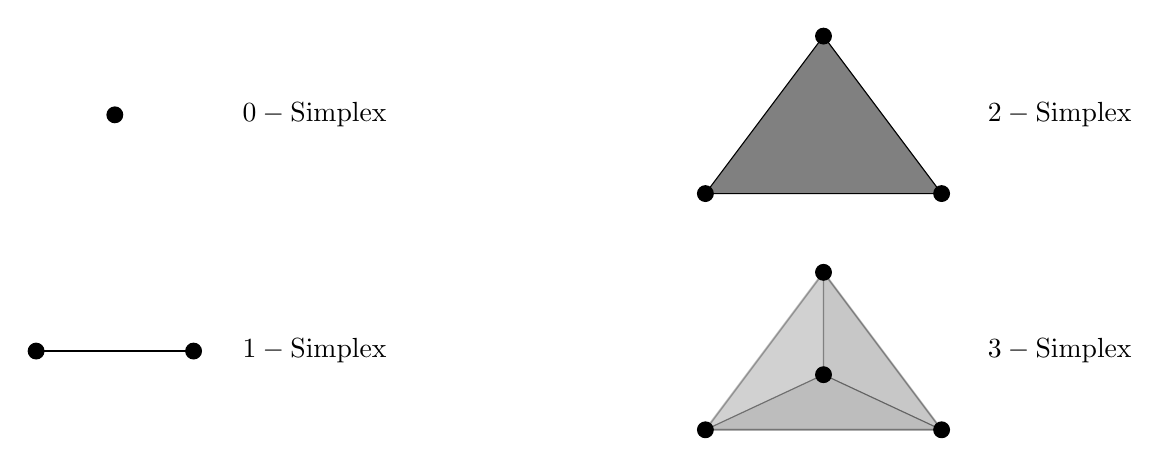
\begin{tikzpicture}
        \filldraw[draw=black,fill=black] (0,1) circle (0.1);
        \node at (1.5,1) [right] {$0-\textrm{Simplex}$};
        \filldraw[draw=black,fill=black] (-1,-2) circle (0.1);
        \filldraw[draw=black,fill=black] (1,-2) circle (0.1);
        \draw[draw=black,semithick] (1,-2) -- (-1,-2);
        \node at (1.5,-2) [right] {$1-\textrm{Simplex}$};
        \filldraw[fill=gray] (9,2) -- (7.5,0) -- (10.5,0) -- cycle;
        \filldraw[draw=black,fill=black] (9,2) circle (0.1);
        \filldraw[draw=black,fill=black] (7.5,0) circle (0.1);
        \filldraw[draw=black,fill=black] (10.5,0) circle (0.1);
        \node at (12,1) {$2-\textrm{Simplex}$};
        \filldraw[draw=black,fill=gray,opacity=0.2] (9,-1) -- (7.5,-3) -- (9,-2.3) -- cycle;
        \filldraw[draw=black,fill=gray,opacity=0.3] (9,-1) -- (10.5,-3) -- (9,-2.3) -- cycle;
        \filldraw[draw=black,fill=gray,opacity=0.4] (9,-2.3) -- (7.5,-3) -- (10.5,-3) -- cycle;
        \filldraw[draw=black,fill=gray,opacity=0.2,thick] (9,-1) -- (7.5,-3) -- (10.5,-3) -- cycle;
        \filldraw[draw=black,fill=black] (9,-1) circle (0.1);
        \filldraw[draw=black,fill=black] (7.5,-3) circle (0.1);
        \filldraw[draw=black,fill=black] (10.5,-3) circle (0.1);
        \filldraw[draw=black,fill=black] (9,-2.3) circle (0.1);
        \node at (12,-2) {$3-\textrm{Simplex}$};
    \end{tikzpicture}
    \caption[Surgery Theory - Simplices]{Examples of Simplices}
    \label{fig:surgery_theory_simplexes}
\end{figure}
A simplicial complex is a set of simplices $\mathcal{H}$ such that the face of any element of $\mathcal{H}$ is also contained in $\mathcal{H}$, and the intersection of two simplices $\sigma_{1},\sigma_{2}\in \mathcal{K}$ is a face of both $\sigma_{1}$ and $\sigma_{2}$.\par
We return to studying surgery exact sequences for $n\geq 5$. Let $\mathcal{M}$ be an $n$ dimensional manifold, and let $G = \pi_{1}(\mathcal{M})$. In our surgery exact sequence we still have this mysterious object $[\mathcal{M},F/Cat]$. Let Cat be either PL or Top. The generalized Poincare Conjecture says that, for $n\geq 5$, $S^{PL}(S^{n}) = S^{Top}(S^{n}) = \{S^{n}\}$. Let $\mathcal{M} = S^{n}$. Then $G = \pi_{1}(\mathcal{M}) = \{e\}$. Then we have the following:
\begin{figure}[H]
    \centering
    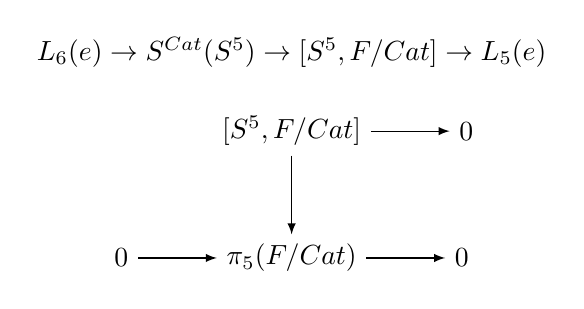
\begin{tikzpicture}[>=latex]
        \node (a) {$[S^{5},F/Cat]$};
        \node (b) [right=of a] {$0$};
        \node (c) [below=of a] {$\pi_{5}(F/Cat)$};
        \node (d) [right=of c] {$0$};
        \node (e) [left=of c] {$0$};
        \node (TEXT) [above=2cm of c] {$L_{6}(e)\rightarrow S^{Cat}(S^{5}) \rightarrow [S^{5},F/Cat] \rightarrow L_{5}(e)$};
        \path[->] (a) edge (b);
        \path[->] (c) edge (d);
        \path[->] (e) edge (c);
        \path[->] (a) edge (c);
    \end{tikzpicture}
    \caption[Surgery Theory - Diagram for Sequence of $S^{5}$]{Digram for the Surgery Exact Sequence of $S^{5}$}
    \label{fig:surgery_theory_example_diagram_for_surgery_exact_sequence}
\end{figure}
So, $\pi_{5}(F/Cat) = \{e\}$. This gives us:
\begin{align*}
    \cdots \rightarrow S^{Cat}(S^{6})\rightarrow [S^{6},F/Cat] &\rightarrow L_{6}(e) \rightarrow \cdots\\
    \cdots &\rightarrow 0 \rightarrow \pi_{6}(F/Cat) \rightarrow \mathbb{Z}_{2}\rightarrow 0
\end{align*}
So, we have $\pi_{6}(F/Cat) \cong \mathbb{Z}_{2}$. In general, $\pi_{n}(F/O) \cong L_{n}(\mathbb{Z})$.
\begin{theorem}[Wall's Theorem]
\begin{equation*}
    L_{n}(\mathbb{Z}) = \begin{cases} \mathbb{Z}, & n \equiv 0 \mod 4 \\ 0, & n \equiv 1 \mod 4 \\ \mathbb{Z}_{2}, & n \equiv 2 \mod 4 \\ 0, & n \equiv 3 \mod 4 \end{cases}
\end{equation*}
\end{theorem}
All $L$ groups are $4$ periodic, and never have odd torsion. That is, there is never $\mathbb{Z}_{3},\mathbb{Z}_{5}$, etc. Wall groups are hard to compute. Whatever $F/Cat$ is, its homotopy groups for $n\geq 5$ are known.
\subsubsection{Principal G-Bundles}
A few things are needed:
\begin{itemize}
    \item Map $p:E\rightarrow X$, where $E$ is a total space and $X$ is a base space.
    \item The inverse-image $E_{x} = p^{-1}(\{x\})$ is called the fiber over $x$.
    \item $G$ (Group) acts on each $E_{x}$ freely and transitively.
    \item $G$ has to act `continuously.' Nearby points are taken to nearby points.
\end{itemize}
Then $p:E\rightarrow X$ is a $G-$principal bundle.
\begin{remark}
Freely means the only element that fixes everything is the identity.
\end{remark}
\begin{example}
Take a sphere $S^{n}$ and a projection $p:S^{n} \rightarrow \mathbb{RP}^{n}$. $\mathbb{RP}^{n}$ is created by glueing antipotal points together. If $x\in \mathbb{RP}^{n}$, then $p^{-1}(\{x\})$ consists of $2$ antipotal points in $S^{n}$. Now $\mathbb{Z}_{2}$ acts on a sphere. $\mathbb{Z}_{2} = \{0,1\}$. $0$ maps $x \mapsto x$ and $1$ maps $x\mapsto -$. Note that $1+1 = 0$, as in $\mathbb{Z}_{2}$. Given any point, you can get to another point in the fiber. This is trivial in this example as there are only two points in the fiber. Also only the identity maps a point back to itself. This action is free and transitive, so $p:S^{n} \rightarrow \mathbb{RP}^{n}$ is a $\mathbb{Z}_{2}$-principal bundle.
\end{example}
\begin{remark}
Let $M$ be a manifold (Or a space) with dimension $n$ and fundamental group $G$. A universal cover $\tilde{M}$ of $M$ is a map $p:\tilde{M}\rightarrow M$ such that $\tilde{M}$ is simply connected of dimension $n$, i.e. $\pi_{1}(\tilde{M}) = e$, and $\forall_{x\in M}$, $p^{-1}(x)$ is a collection of discrete points.
\end{remark}
\begin{remark}
$\pi_{1}(\mathbb{RP}^{n}) = \mathbb{Z}_{2}$ and $S^{n}$ is a universal cover of $\mathbb{RP}^{n}$. So this might come from a general theory.
\end{remark}
\begin{example}
Take the circle $S^{1}$. $\pi_{1}(S^{1}) = \mathbb{Z}$. There's a map $p(x) = e^{2\pi i x}$ of modulus $1$. Note that $p^{-1}(0) = \mathbb{Z}$. So $p^{-1}(x)$ is just a shift of $\mathbb{Z}$ $(\mathbb{Z}+r)$. Note that $\pi_{1}(\mathbb{R}) = e$. So $\mathbb{R}$ is a universal cover of $S^{1}$.
\end{example}
\begin{example}
We may think $\mathbb{R}^2$ is a universal cover of $S^{2}$, but $S^{2}$ is already simply connected. So $p$ is simply the identity map, and the universal cover of $S^{2}$ is simply $S^{2}$. All universal covers are homotopy equivalent.
\end{example}
\begin{remark}
Let $x\in M$. Then, for all $z\in p^{-1}(\{x\})$, and for all $g\in \pi_{1}(M)$, there is an action $gx\in p^{-1}(x)$. This uses the homotopy lifting property.
\end{remark}
There is an action $G$ on $\tilde{M}$ which preserves the fiber (Takes every element of a fiber to the same fiber. That is, it does not mix fibers), is transitive, and is free. The map $p:\tilde{M}\rightarrow M$ is a $\pi_{1}(M)-$Principal Bundle.
\subsubsection{Functors}
Let $F$ be a functor $F:\textit{Space}\rightarrow \textit{Groups}$. So for all spaces $X$, we have a group $F(X)$. There are many such examples:
\begin{itemize}
    \begin{multicols}{4}
        \item Cohomology
        \item Homology
        \item K-Theory
        \item Other Stuff
    \end{multicols}
\end{itemize}
\begin{remark}
Homology: Take $M$ and triangulate. Take maps from the simplicial complex of $M$ to $G$ (Group) (Certain conditions). There's an equivalence relation on these maps. That set after taking the equivalence relations is the homology: $H_{n}(M,G)$. $n$ describes the type of simplicies. If $n > \dim(M)$, then $H_{n}(G,M) = 0$. $H_{n}(M,G) = \{f:\Delta^{n}\rightarrow G\}$.
\end{remark}
We want to talk about cohomology. Under special conditions there is something called the Brown Representation Theorem. Consider Cohomology $H^{n}(M,G)$, with coefficients in $G$. Cohomology is Homotopy invariant, that is if $M \simeq N$, then $H^{n}(M,G) \simeq H^{n}(N,G)$. The Brown-Representation Theorem says that there is a classifying space $BG$ such that, for all spaces $M$, there is a one-to-one correspondence between $H^{n}(X,G) \leftrightarrow [X,K(G,n)]$. In general, if $F$ is a functor, then the Brown-Representation Theorem says that there is a classifying space $Y$ such that $F(X)$ has a one-to-one correspondence with the homotopy classes of maps, $[X,Y]$. $F(x) \leftrightarrow [X,Y]$
\begin{example}
The Eilenberg-MacLane Space $K(G,n)$ has the property that, for all $j\ne n$, $\pi_{n}(K(G,n)) = G$, and $\pi_{j}(K(G,n)) = 0$. $K(G,n)$ is the classifying space for cohomology.
\end{example}
\begin{theorem}
$K(G,n)$ is the classifying space for cohomology. That is, up to homotopy, $H^{n}(X,G) \leftrightarrow [X,K(G,n)]$.
\end{theorem}
Let $\textrm{Prin}_{G}(X)$ be the collection of $G-$principal bundles on $X$. With a certain equivalence relation, it turns out the $\textrm{Prin}_{G}(X)$ is a group. So $\textrm{Prin}_{G}:\textit{Spaces}\rightarrow \textit{Groups}$ is a functor. The Brown-Representation Theorem implies that there is a classifying space $BG$ $\textrm{Prin}_{G}\leftrightarrow [X,BG]$.
\begin{theorem}
If $p:E\rightarrow X$ and $p':E'\rightarrow X$ are both bundles over $X$, then there exists $p\oplus p':E\oplus E' \rightarrow X$ COME BACK TO LATER
\end{theorem}
\subsubsection{Grothendieck Groupification of Semigroup}
\begin{definition}
A semi-group is a group without the requirement for invereses.
\end{definition}
\begin{example}
$\{0,1,2,\hdots\}$ is a semi-group under addition.
\end{example}
Let $G$ be a semi-group. Constraint $G\times G/\sim$. $(a,b) \sim (c,d)$ if $a+d = b+c$. So, $(2,3)\sim (4,5) \sim (7,8)\sim (-1,0) \equiv -1$. The equivalence class of all of these things is called $-1$. We still have all of the positive integers, $(4,2)\sim(5,3) \sim(6,4) \equiv 2$. This process adds all of the negatives. This process, called Grothendique Construction on a Semi-group creates a group out of a semi-group. It is, in a way, the 'smallest' group containing the semi-group. The groupification of $\{0,1,2,3,\hdots\}$ will be $\mathbb{Z}$.
\begin{example}
What are the vector bundles over a dot? THere is $\mathbb{R}^{0}$ (A dot), $\mathbb{R}^{n}, \hdots,\mathbb{R}^n,\hdots $. There is an operation on this set $\{\mathbb{R}^{n}:n \geq 0\}$. This makes a semi-group, and there is a Grothendique Groupification $G_{r}(\mathbb{Z}_{\geq 0}, +) = \mathbb{Z}$
\end{example}
\clearpage
\printglossaries
\end{document}